% THIS DOCUMENT IS FOLLOWS THE VOLERE TEMPLATE BY Suzanne Robertson and James Robertson
% ONLY THE SECTION HEADINGS ARE PROVIDED
%
% Initial draft from https://github.com/Dieblich/volere
%
% Risks are removed because they are covered by the Hazard Analysis
\documentclass[12pt]{article}

\usepackage{booktabs}
\usepackage{tabularx}
\usepackage{hyperref}
\usepackage{graphicx}
\usepackage{array}
\graphicspath{ {./diagrams/} }
\hypersetup{
    bookmarks=true,         % show bookmarks bar?
      colorlinks=true,      % false: boxed links; true: colored links
    linkcolor=red,          % color of internal links (change box color with linkbordercolor)
    citecolor=green,        % color of links to bibliography
    filecolor=magenta,      % color of file links
    urlcolor=cyan           % color of external links
}

\newcommand{\lips}{\textit{Insert your content here.}}

%% Comments

\usepackage{color}

\newif\ifcomments\commentstrue %displays comments
%\newif\ifcomments\commentsfalse %so that comments do not display

\ifcomments
\newcommand{\authornote}[3]{\textcolor{#1}{[#3 ---#2]}}
\newcommand{\todo}[1]{\textcolor{red}{[TODO: #1]}}
\else
\newcommand{\authornote}[3]{}
\newcommand{\todo}[1]{}
\fi

\newcommand{\wss}[1]{\authornote{blue}{SS}{#1}} 
\newcommand{\plt}[1]{\authornote{magenta}{TPLT}{#1}} %For explanation of the template
\newcommand{\an}[1]{\authornote{cyan}{Author}{#1}}

%% Common Parts

\newcommand{\progname}{Software Engineering} % PUT YOUR PROGRAM NAME HERE
\newcommand{\authname}{Team 8 -- Rhythm Rangers\\
\\ Ansel Chen
\\ Muhammad Jawad
\\ Mohamad-Hassan Bahsoun
\\ Matthew Baleanu
\\ Ahmed Al-Hayali} % AUTHOR NAMES                  

\usepackage{hyperref}
    \hypersetup{colorlinks=true, linkcolor=blue, citecolor=blue, filecolor=blue,
                urlcolor=blue, unicode=false}
    \urlstyle{same}
                                


\begin{document}

\title{Software Requirements Specification for \progname: subtitle describing software} 
\author{\authname}
\date{\today}
	
\maketitle

~\newpage

\pagenumbering{roman}

\tableofcontents

~\newpage

\section*{Revision History}

\begin{tabularx}{\textwidth}{p{3cm}p{2cm}X}
\toprule {\textbf{Date}} & {\textbf{Version}} & {\textbf{Notes}}\\
\midrule
Date 1 & 1.0 & Notes\\
Date 2 & 1.1 & Notes\\
\bottomrule
\end{tabularx}

~\\

~\newpage
\section{Purpose of the Project}
\subsection{User Business}
\lips
\subsection{Goals of the Project}
\lips
\section{Stakeholders}
\subsection{Client}
\lips
\subsection{Customer}
\lips
\subsection{Other Stakeholders}
\lips
\subsection{Hands-On Users of the Project}
\lips
\subsection{Personas}
\lips
\subsection{Priorities Assigned to Users}
\lips
\subsection{User Participation}
\lips
\subsection{Maintenance Users and Service Technicians}
\lips

\section{Mandated Constraints}
\subsection{Solution Constraints}
\begin{itemize}

  \item The service uses a music dataset
  \\ \textbf{Rationale:} A dataset for an AI project is necessary as some form of training data must be used 
  in order to train the AI generative, analysis and recommendation systems. 
  \\ \textbf{Fit Criterion:} The machine learning algorithms use a music dataset as the training set. 

  \item The service uses a machine learning algorithm in order to generate song recommendations and snippets. 
  \\ \textbf{Rationale:} The general gist of this project is a leveraging of different signal processing and machine learning
  algorithms in order to provide an end user with a better experience for consuming music. We believe that using a machine 
  learning algorithm for these ends would both be interesting in terms of implementing and training a model, but also practically
  useful for the end user to provide better recommendations by leveraging training over a very large dataset in order to produce results. 
  \\\textbf{Fit Criterion:} The recommendation and generation components utilize trained machine learning algorithm. 

  \item The service features integration with an existing music streaming provider's platform. 
  \\ \textbf{Rationale:} A music service provider (such as Spotify) would allow the service to bypass the need to have
  music inputted, instead being able to use references to a track. In addition, through API calls, providers such as spotify
  already have a large amount of useful labels for invidiual track(s) that can be used as features for the machine learning
  components of the service.  
  \\ \textbf{Fit Criterion:} The service has components that make uses of features (such as API calls) 
  that belong to a music service provider's platform. 

  \item The service uses a server to process the user requests separately from the front end.
  \\ \textbf{Rationale:} Ideally, our service would use an on-premise deployed ubuntu server in order to process the user 
  analysis, recommendation, and generation components of the project, as this would allow a more flexible front end design
  (such as through a web application). 
  \\ \textbf{Fit Criterion:} An on-premise server is deployed for the purposes of handling the analysis, generation and recommendations
  systems separately from the front end. 

\end{itemize}

\subsection{Implementation Environment of the Current System}
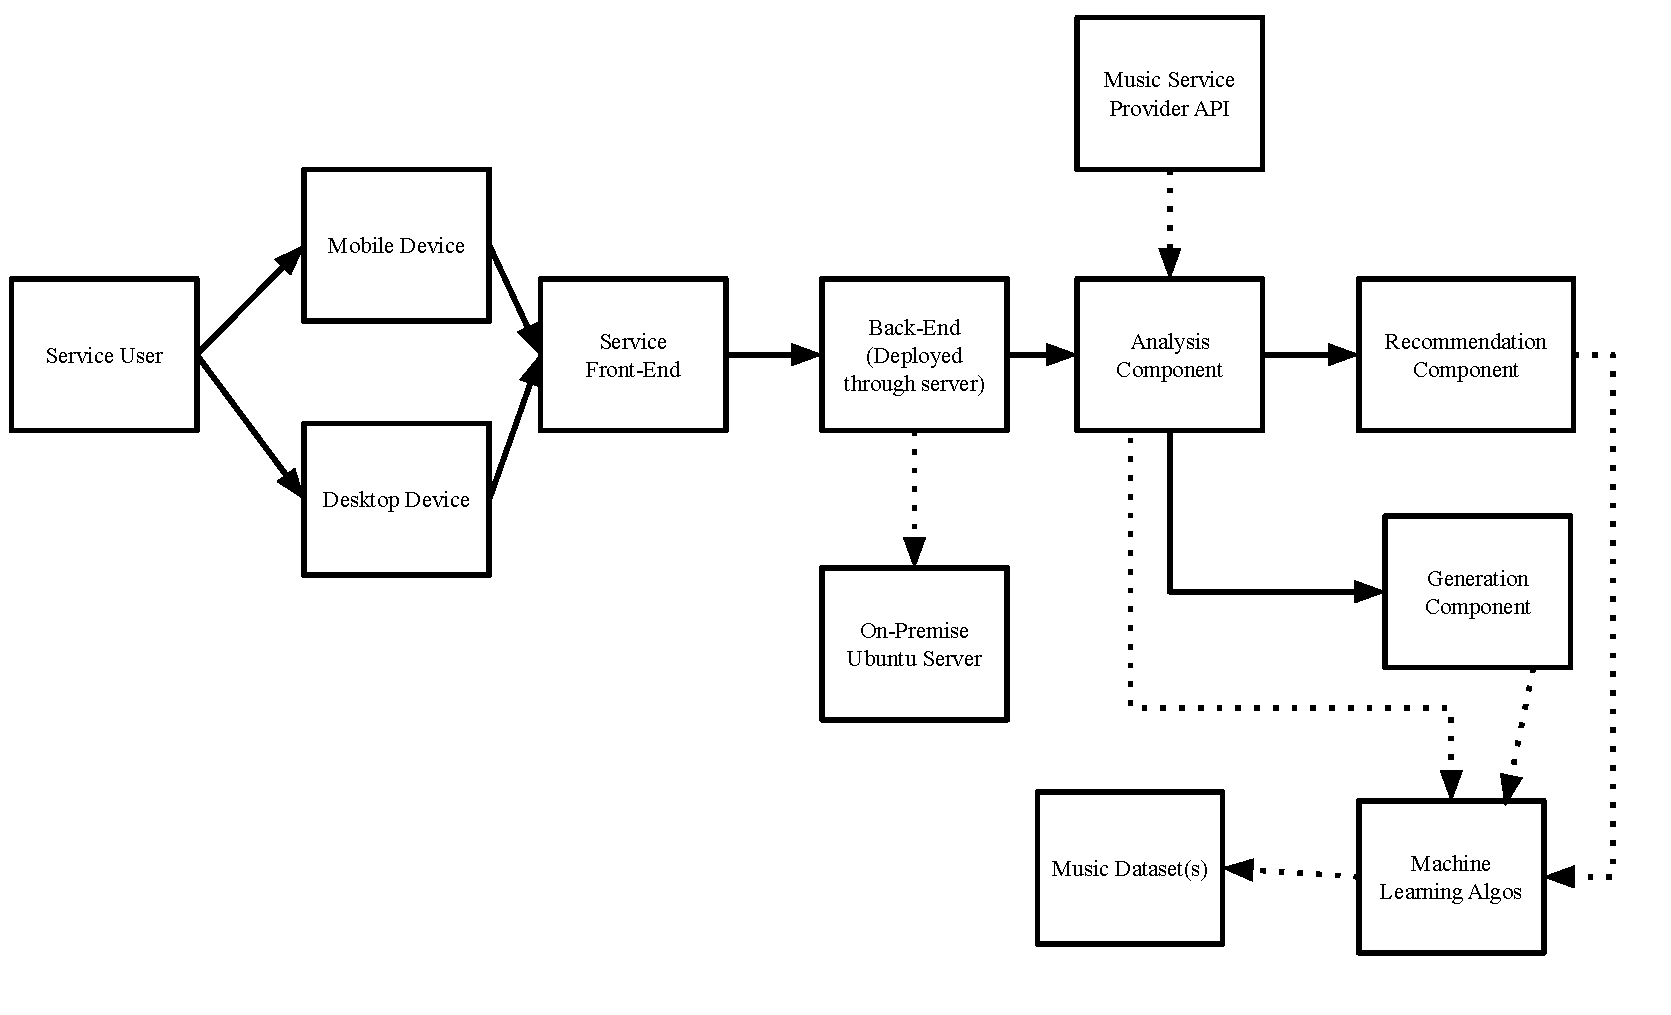
\includegraphics[scale=0.552]{3_2_environment_diagram.pdf}

\subsection{Partner or Collaborative Applications}
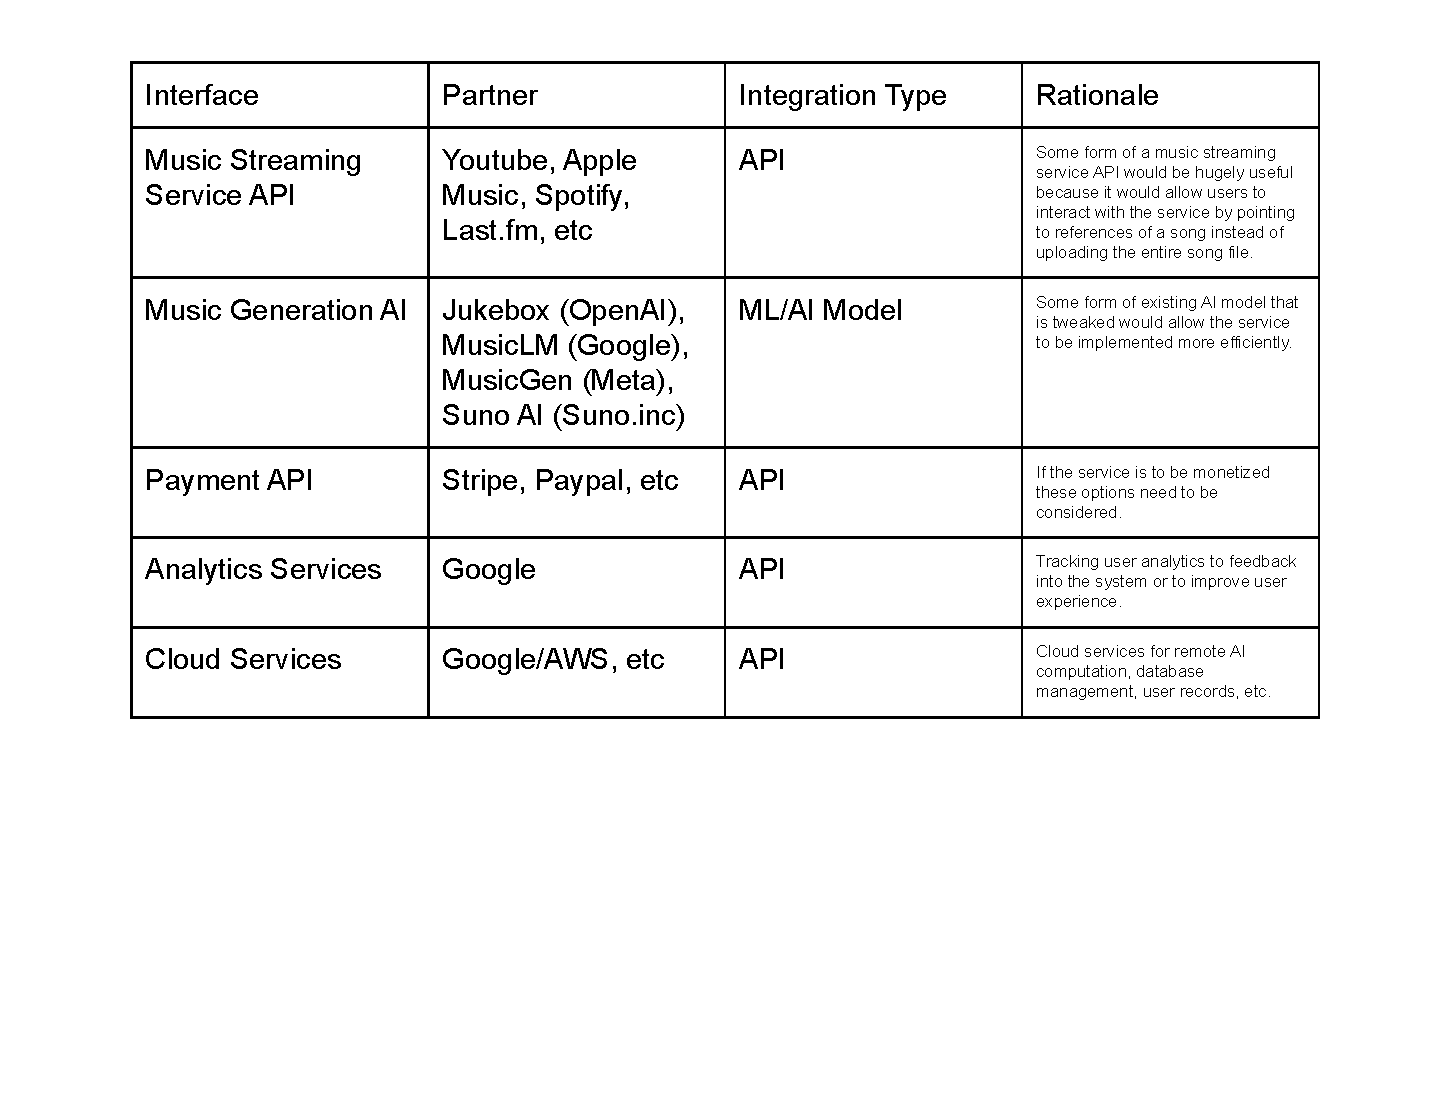
\includegraphics[scale=0.72]{3_3_partner_constraints_figure}

\subsection{Off-the-Shelf Software}
There are several existing solutions that could serve as part of the music generation and recommendation system. These include:

\begin{itemize}
    \item \textbf{Spotify API}: Provides access to a vast library of music, including song previews and metadata, which can be leveraged for generating recommendations.
    \item \textbf{Librosa Library}: An open-source Python package for analyzing and processing music files, suitable for extracting features from songs and facilitating generative components.
    \item \textbf{TensorFlow and PyTorch Pre-trained Models}: Both frameworks offer pre-trained models that could be adapted for music generation tasks. These solutions provide a basis for deep learning models without having to build and train from scratch.
    \item \textbf{OpenAI Jukebox}: A generative model that is capable of producing music, which could potentially be adapted and integrated into our system.
\end{itemize}

These off-the-shelf software solutions provide a foundation upon which we can build our custom features, significantly reducing the development time and leveraging existing technologies to enhance the functionality of our platform.

\subsection{Anticipated Workplace Environment}
\begin{itemize}
  \item Home Usage
  \\\textbf{Rationale:} This environment is more appropriate for casual music listeners. 
  This means users will most likely be using it in a form of a casual environment. This can 
  include such as during a public commute on the train, where the user might try to interact 
  with the service while there is an unreliable internet connection on a mobile device. This
  means the front end of the service must be easy to use and access on all types of devices, 
  and preferrably, not a large amount of data is streamed between the user and the service. 
  This means that preferrably, the input would have references to pieces of music instead of 
  having say, full .MP3 files as the input. These users are also more likely interested in the 
  recommendation system to attempt to find new pieces of music to listen to, and might be more
  willing to use the generation system for "fun", so they might be satifisfied even with a 
  generation component that produces odd results.
 
  \item Studio Usage
  \\\textbf{Rationale:} This environment is more professional and what is most likely what 
  creative professionals will be using. The expectation is that they will be using this on their 
  computers, thus they are more likely have a reliable internet connection in addition to being
  willing to input a lot more music to the service. This means that the service needs to faciliate 
  entering a large amount of music, and be able to generate results in a rapid and efficient 
  manner. Because the users of this type of environment would likely be inviduals engaged in some form
  of creative endeavors, they will generally have higher standards of what the service provides, and
  might be more interested in the analysis component, such as being able to find new labels for their
  existing work to get new perspectives. This also means that they most likely expect the music generation
  component to give them something more "listenable", something they could directly use as a sample or inspiration.  

\end{itemize}

\subsection{Schedule Constraints}
This project was started in the 2024 Fall Term and is expected to be completed by the 
2025 winter term at McMaster university. Some of the key deadlines are: 
\begin{itemize}
  \item Proof of Concept Demonstration Plan, November 11-22
  \\This deadline accounts for 5\% of the mark. The group should have identified the most significant
  risks involving the project and come up with plans on how to migitate said risks. If this is not possible, then the project 
  can be redefined. The group also needs to predict and note other concerns about potential problems or difficulties that could arise
  during development, such as testing difficulties or software portability. If this deadline is not met, then it means that our group
   does not fully understand the potential pitfalls of our project and we need to redefine certain aspects of the project. 

  \item Final Demonstration, March 24-30
  \\This deadline accounts for 20\% of the mark. This deadline involves a demonstration of a finalized 
  version of the project to supervisors before the public EXPO happening at a TBD date. By this deadline, 
  the service should be in a completed state ready for use and demonstration. If this deadline is not met then
  the project can be considered a "failure". 

  \item Final Documentation, April 2
  \\This deadline accounts for 30\% of the mark. It involves the finalized documentation of plans pertaining to 
  the project and the actual working program/service. Any final revisions and reflections pertaining to the project
  should have been completed by this deadline as no further changes to the project will be possible. Whatever documentation
  or code that is not completed by this deadline would be considered permanently unfinished. 
\end{itemize}

\subsection{Budget Constraints}
The budget limit as stated by the capstone outline is 750\$ CAD. Potential additional
costs might include API calls, software liscensing, account fees for cloud services. 
For the purposes of the demonstration they should not exceed the 750\$ limit. 

\subsection{Enterprise Constraints}
There are no specific enterprise constraints as we do not have outside investors
for this project. 

\section{Naming Conventions and Terminology}
\subsection{Glossary of All Terms, Including Acronyms, Used by Stakeholders
involved in the Project}
\lips

\section{Relevant Facts And Assumptions}
\subsection{Relevant Facts}
\begin{itemize}
  \item Music contains the following core features \begin{itemize}
    \item Tempo
    \item Key signature
    \item Time signature
    \item Pitch
    \item Timbre
  \end{itemize}
  \item Song files have metadata that contains information such as: \begin{itemize}
    \item Song title
    \item Artist
    \item Release date
  \end{itemize}
  \item Most songs can be classified into multiple genres
\end{itemize}
\subsection{Business Rules}
\begin{itemize}
  \item The user should be able to generate their own music
  \item The user should be able to figure out what musical features a song contains 
  \item The user should be able to ask for similar songs
  \item the user should be able to interact with the system without any external installation
\end{itemize}
\subsection{Assumptions}
\begin{itemize}
  \item Users will have at least some familiarity of music theory
  \item The analysis and recommendation systems will use as many well-established musical 
  features as possible
  \item All API inputs will be easily accessible and reliable enough to support the
  recommendation and analysis systems
  \item The system will be written in a language that all developers are familiar with
  \item The system will use a local server to handle the processing of
  the machine learning model and large datasets
  \item Handling of niche features and cover art are designed to enhance the user experience, but 
  these will not be a part of the core functionality of the system
  \item The generative system will be completed by the POC demo date
  \item The recommendation and analysis systems will be completed by the Revision 0 date
\end{itemize}

\section{The Scope of the Work}
\subsection{The Current Situation}
\lips
\subsection{The Context of the Work}
\lips
\subsection{Work Partitioning}
\lips
\subsection{Specifying a Business Use Case (BUC)}
\lips

\section{Business Data Model and Data Dictionary}
\subsection{Business Data Model}
\lips
\subsection{Data Dictionary}
\lips

\section{The Scope of the Product}
\subsection{Product Boundary}
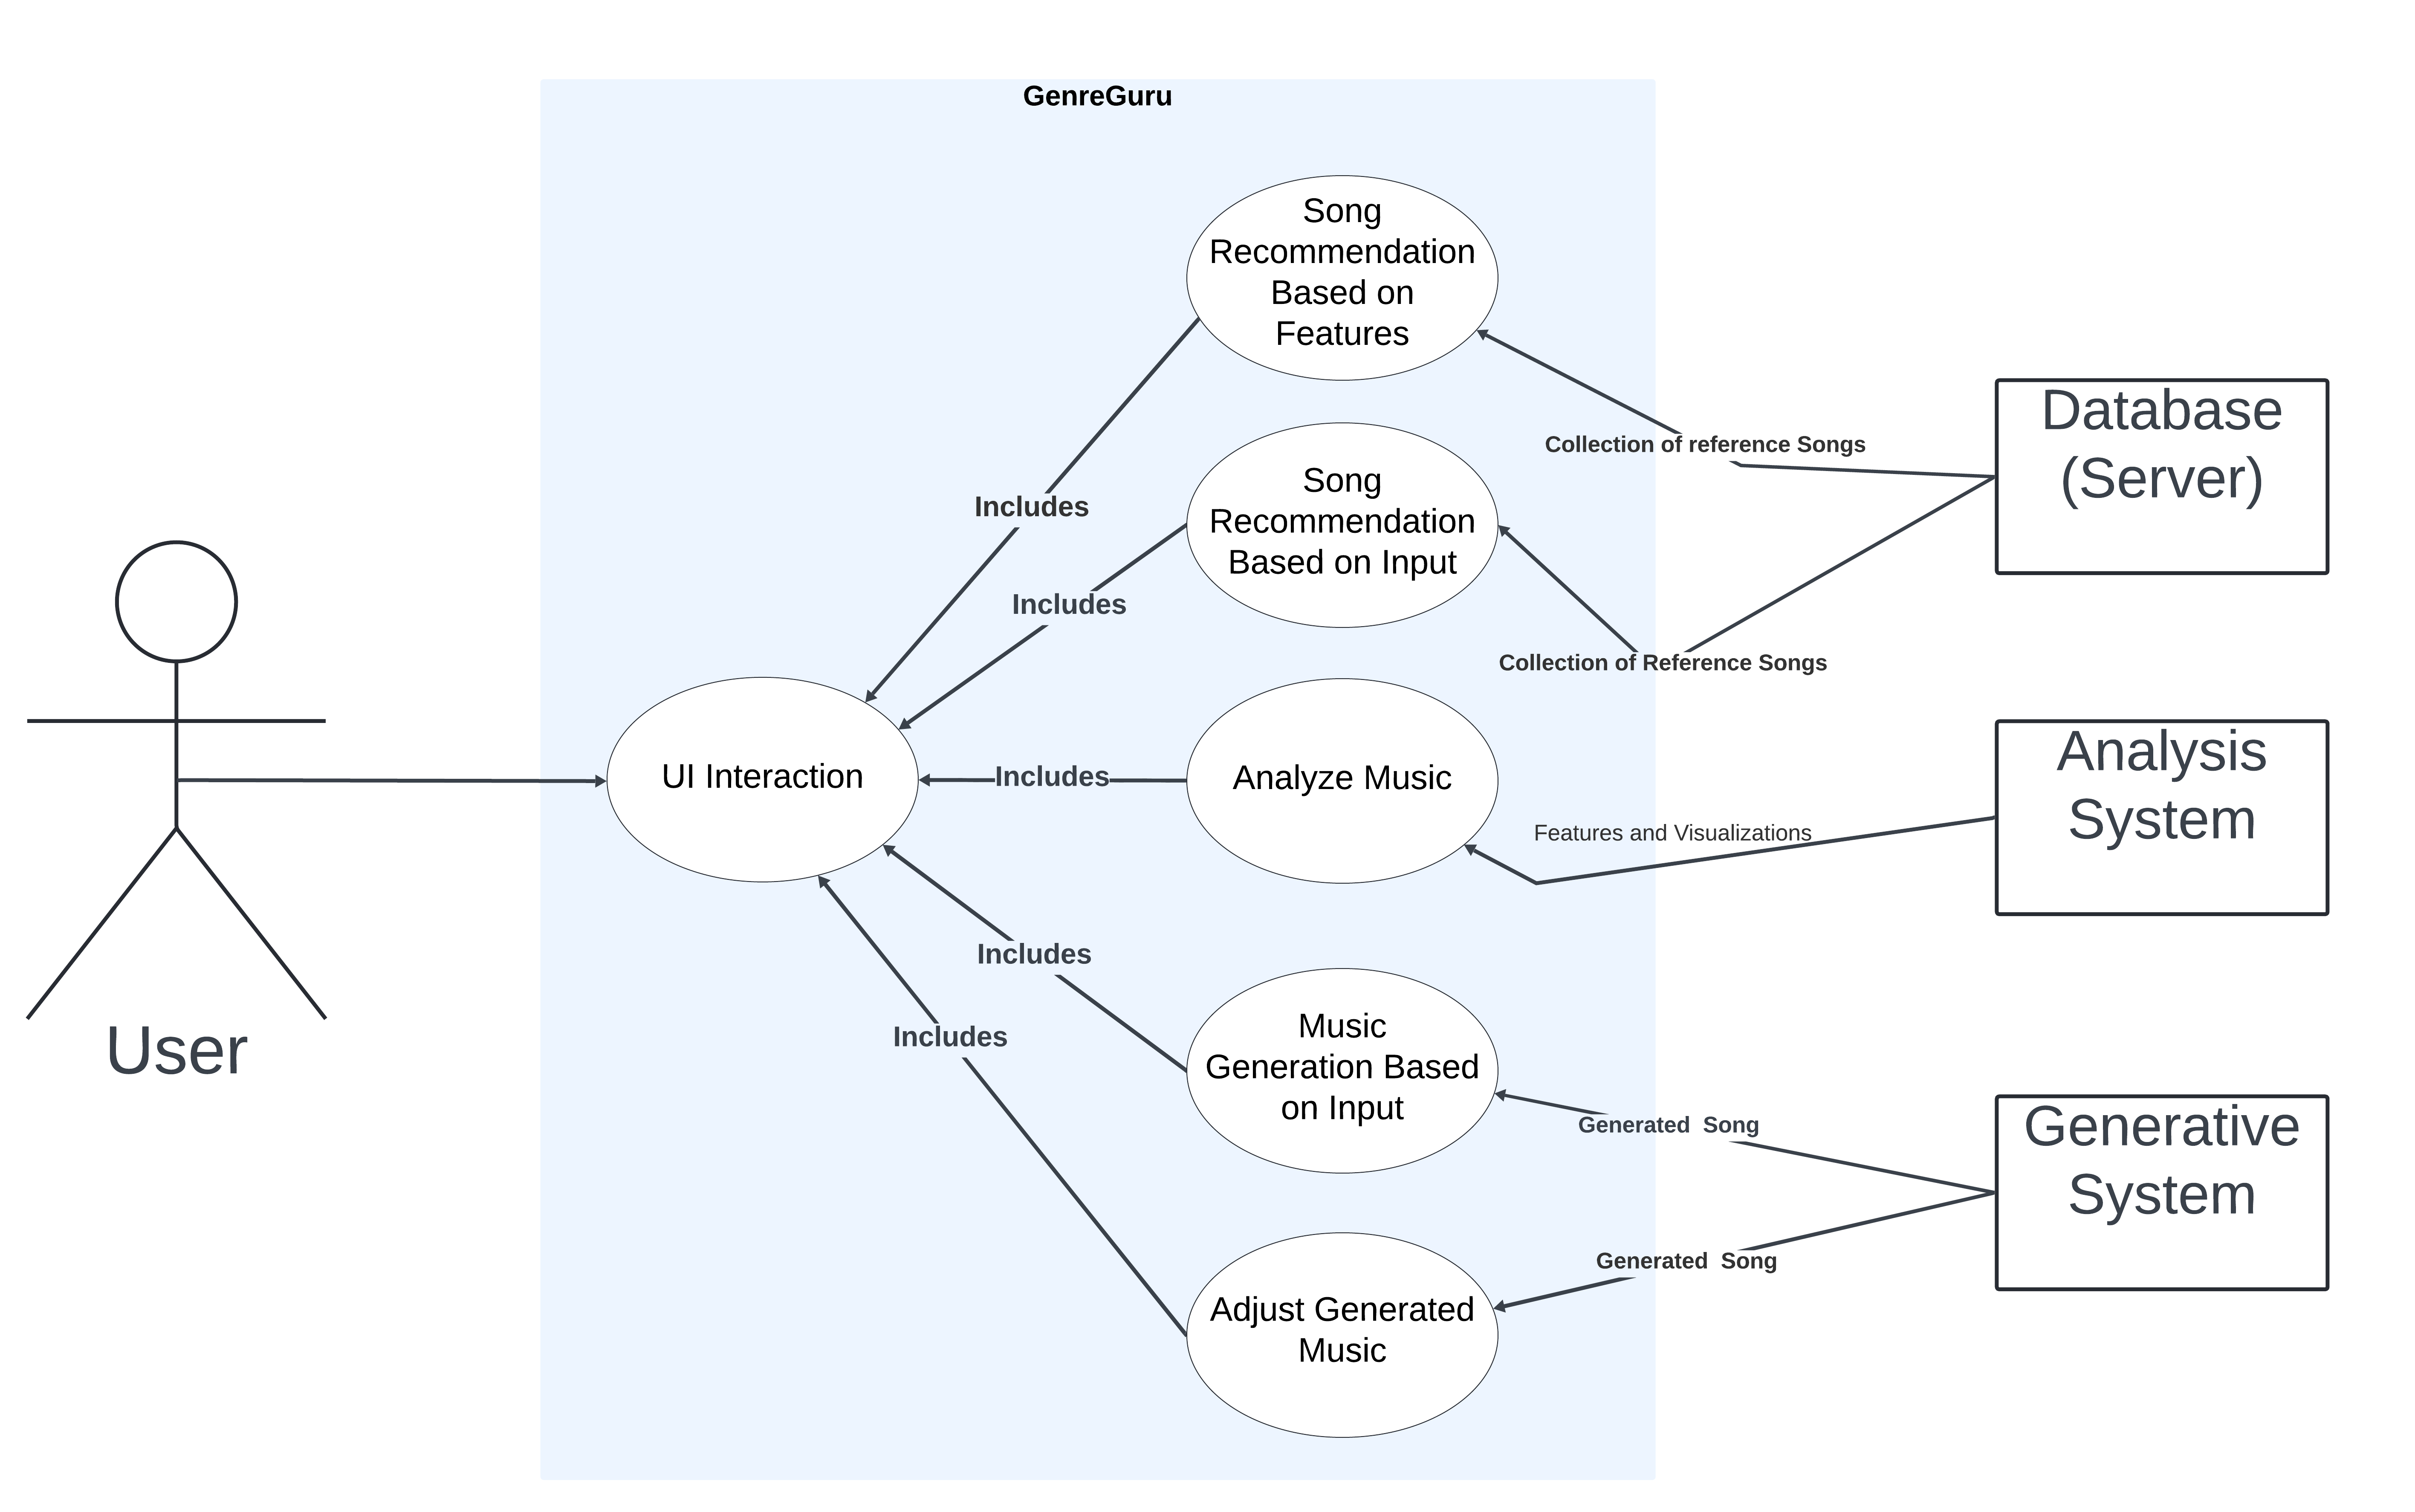
\includegraphics[width=\textwidth]{product_boundary.png} \\
\subsection{Product Use Case Table}
\begin{table}[!ht]
    \centering
    \resizebox{\textwidth}{!}{
    \begin{tabular}{|l|l|l|l|}
    \hline
        \textbf{PUC No} & \textbf{PUC Name} & \textbf{Actor/s} & \textbf{Input \& Output} \\ \hline
        1 & UI Interaction & User & User Actions (click, swipe, drag) (in) \newline System Response (out) \\ \hline
        2 & Song Recommendation Based on Features & User & User's desired features (in) \newline Collection of reference songs (out) \\ \hline
        3 & Music Generation Based on Input & User & Reference song(s) and/or song snippet(s) (in) \newline Generated song or song snippet (out) \\ \hline
        4 & Analyze Music & User & Reference song or song snippet (in) \newline Collection of features and visualizations (out) \\ \hline
        5 & Song Recommendation Based on Input & User & Reference song(s) (in) \newline Collection of reference songs (out) \\ \hline
        6 & Server Interaction for Music Generation & Server & Reference song(s) and/or song snippet(s) (in) \newline Generated song or song snippet (out) \\ \hline
        7 & Server Interaction for Song Recommendation & Server & User's desired features or reference song(s) and/or snippet(s) (in) \newline Collection of reference songs (out) \\ \hline
        8 & Server Interaction for Music Analysis & Server & Reference song or song snippet (in) \newline Collection of features and visualizations (out) \\ \hline
    \end{tabular}
    }
    \caption{Product Use Case Table}
    \label{tab:PUCtable}
\end{table}

\subsection{Individual Product Use Cases (PUC's)}
\textbf{1. Product Use Case Name:} UI Interaction \\
\textbf{Trigger:} User commits some action (e.g. clicking, swiping, dragging) \\
\textbf{Preconditions:} User has successfully accessed GenreGuru, or is already in GenreGuru \\
\textbf{Interested Stakeholders:} All \\
\textbf{Actor/s:} User \\
\textbf{Activity Diagram:} \\
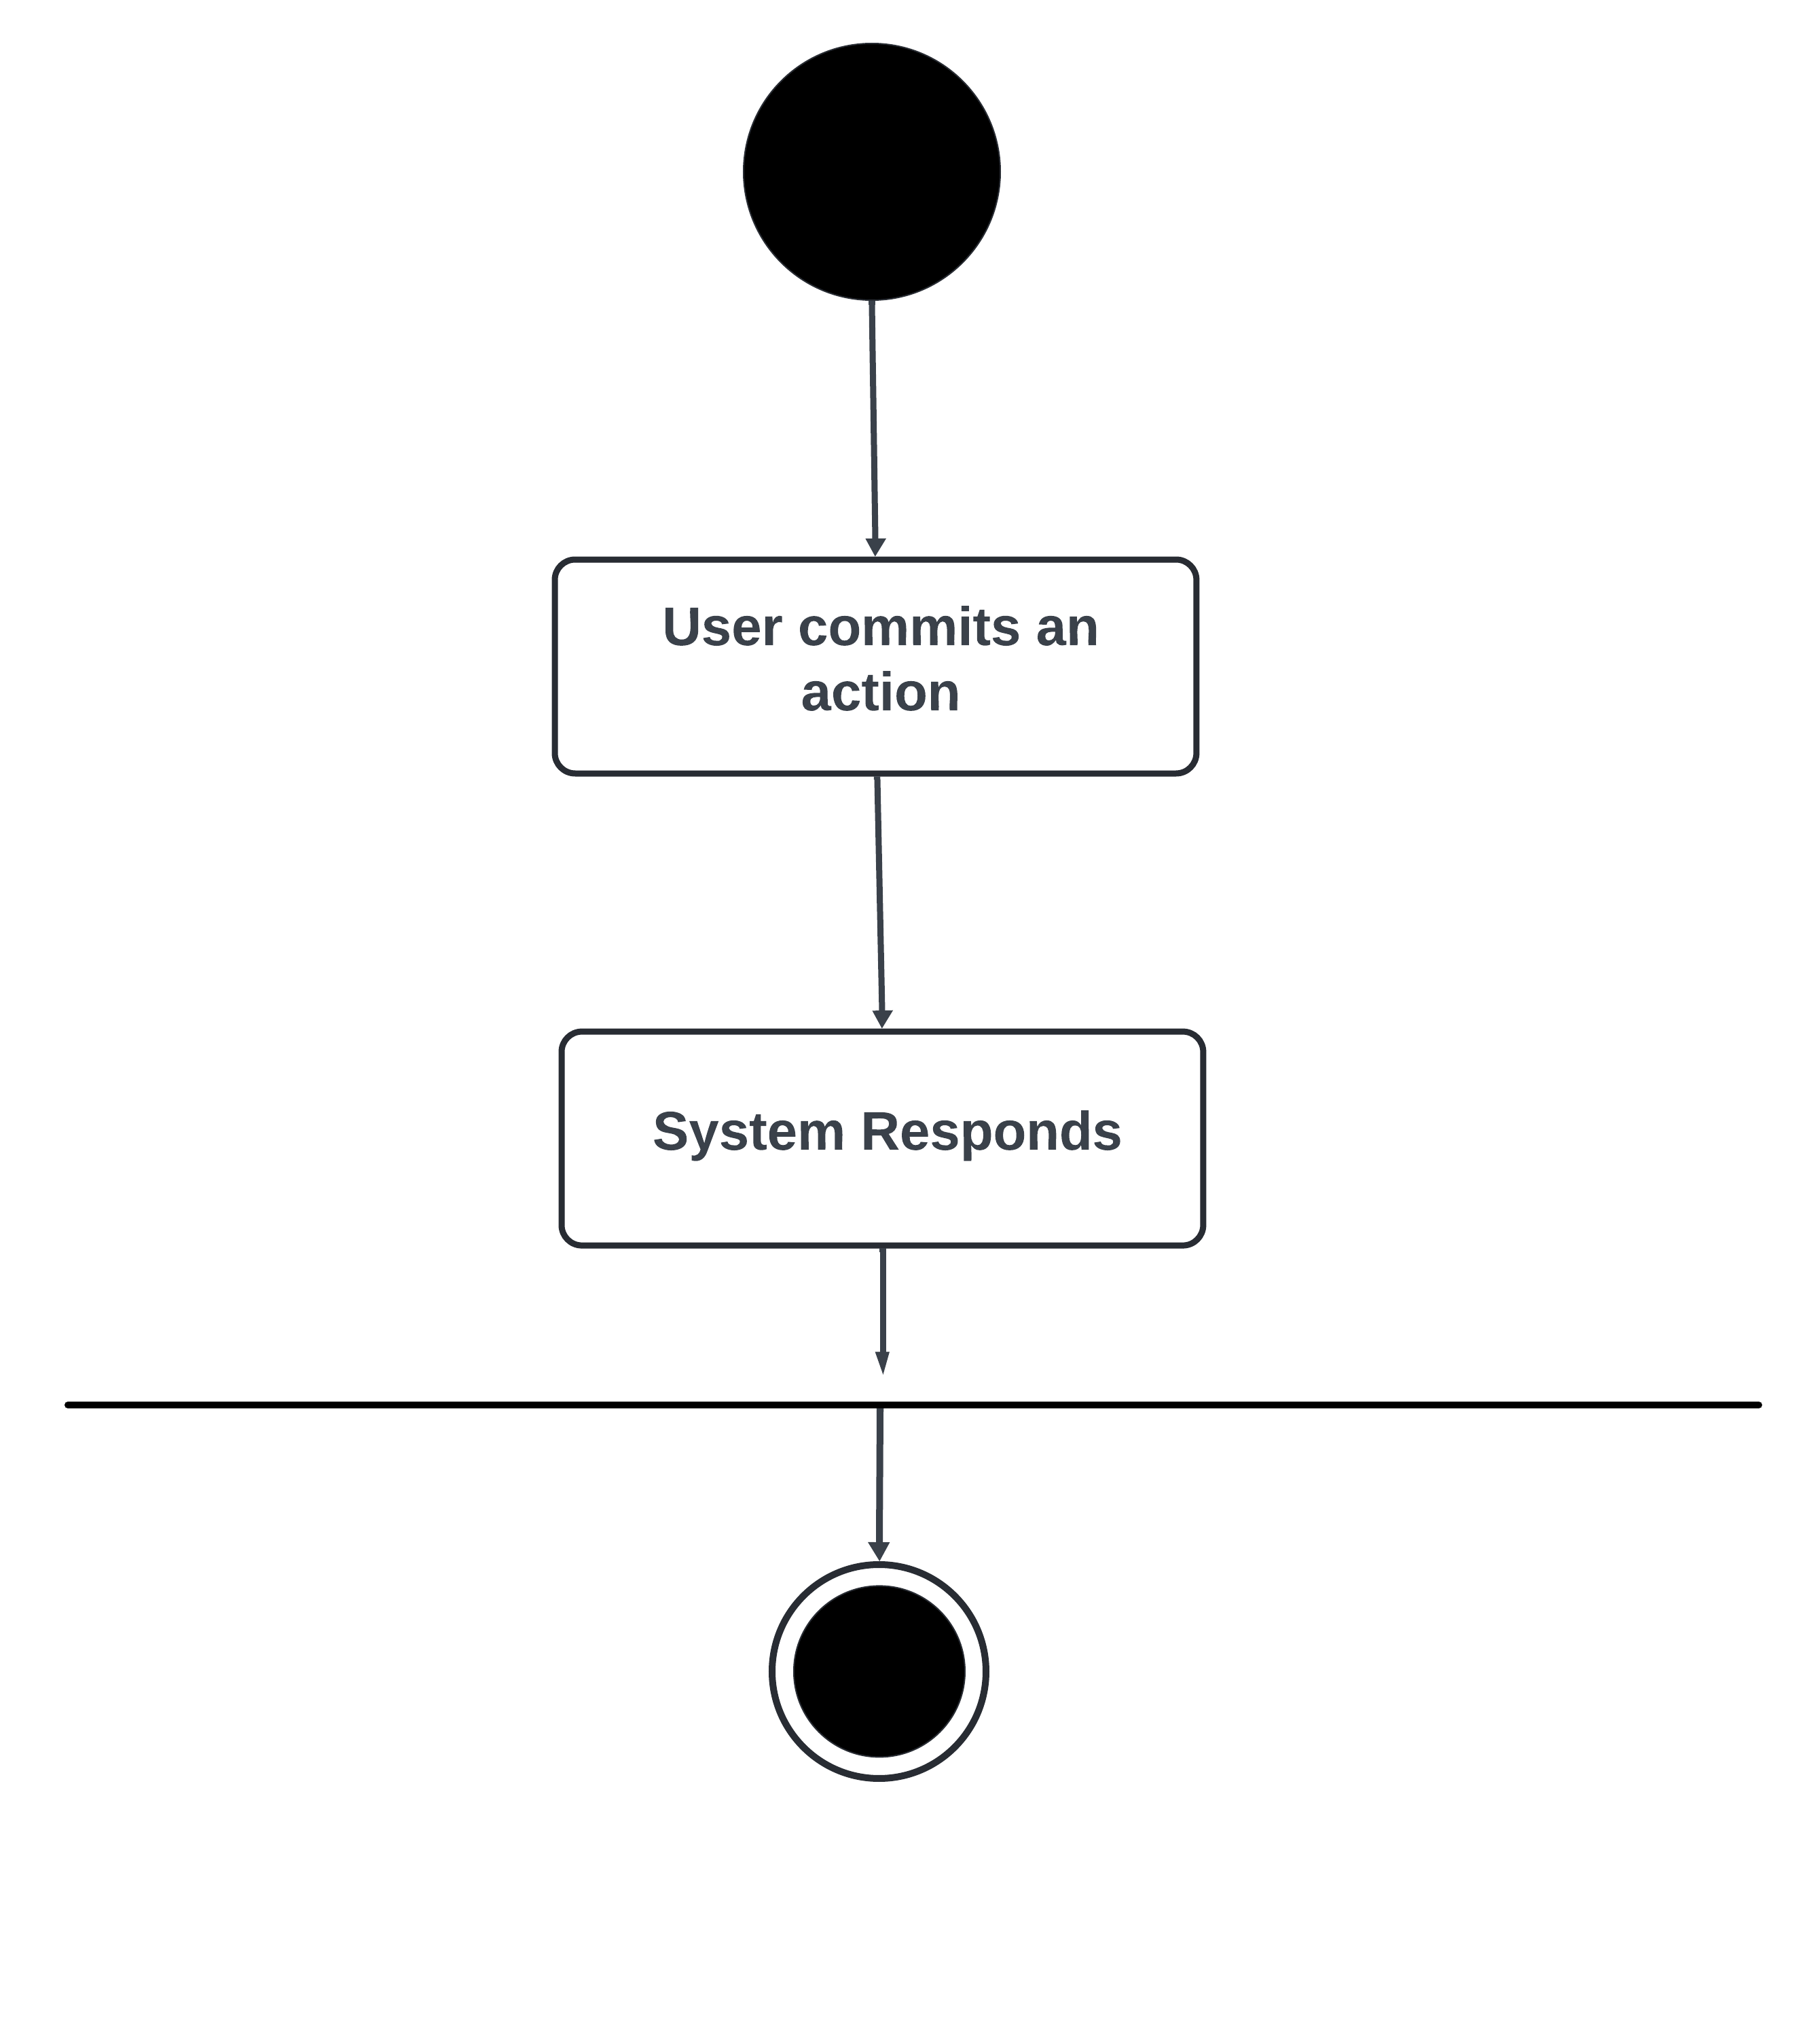
\includegraphics[width=\textwidth]{UI.png} \\
\textbf{Outcome:} The user will commit an action like swiping or pressing and the system will react depending on the action.

\vspace{1cm}

\noindent \textbf{2. Product Use Case Name:} Song Recommendation Based on Features \\
\textbf{Trigger:} User picks features, and indicates they want to search for recommendations \\
\textbf{Preconditions:} User must have GenreGuru open, the user has selected features to search for \\
\textbf{Interested Stakeholders:} Casual Music Listeners, Hobbyist Musicians \\
\textbf{Actor/s:} User \\
\textbf{Activity Diagram:} \\
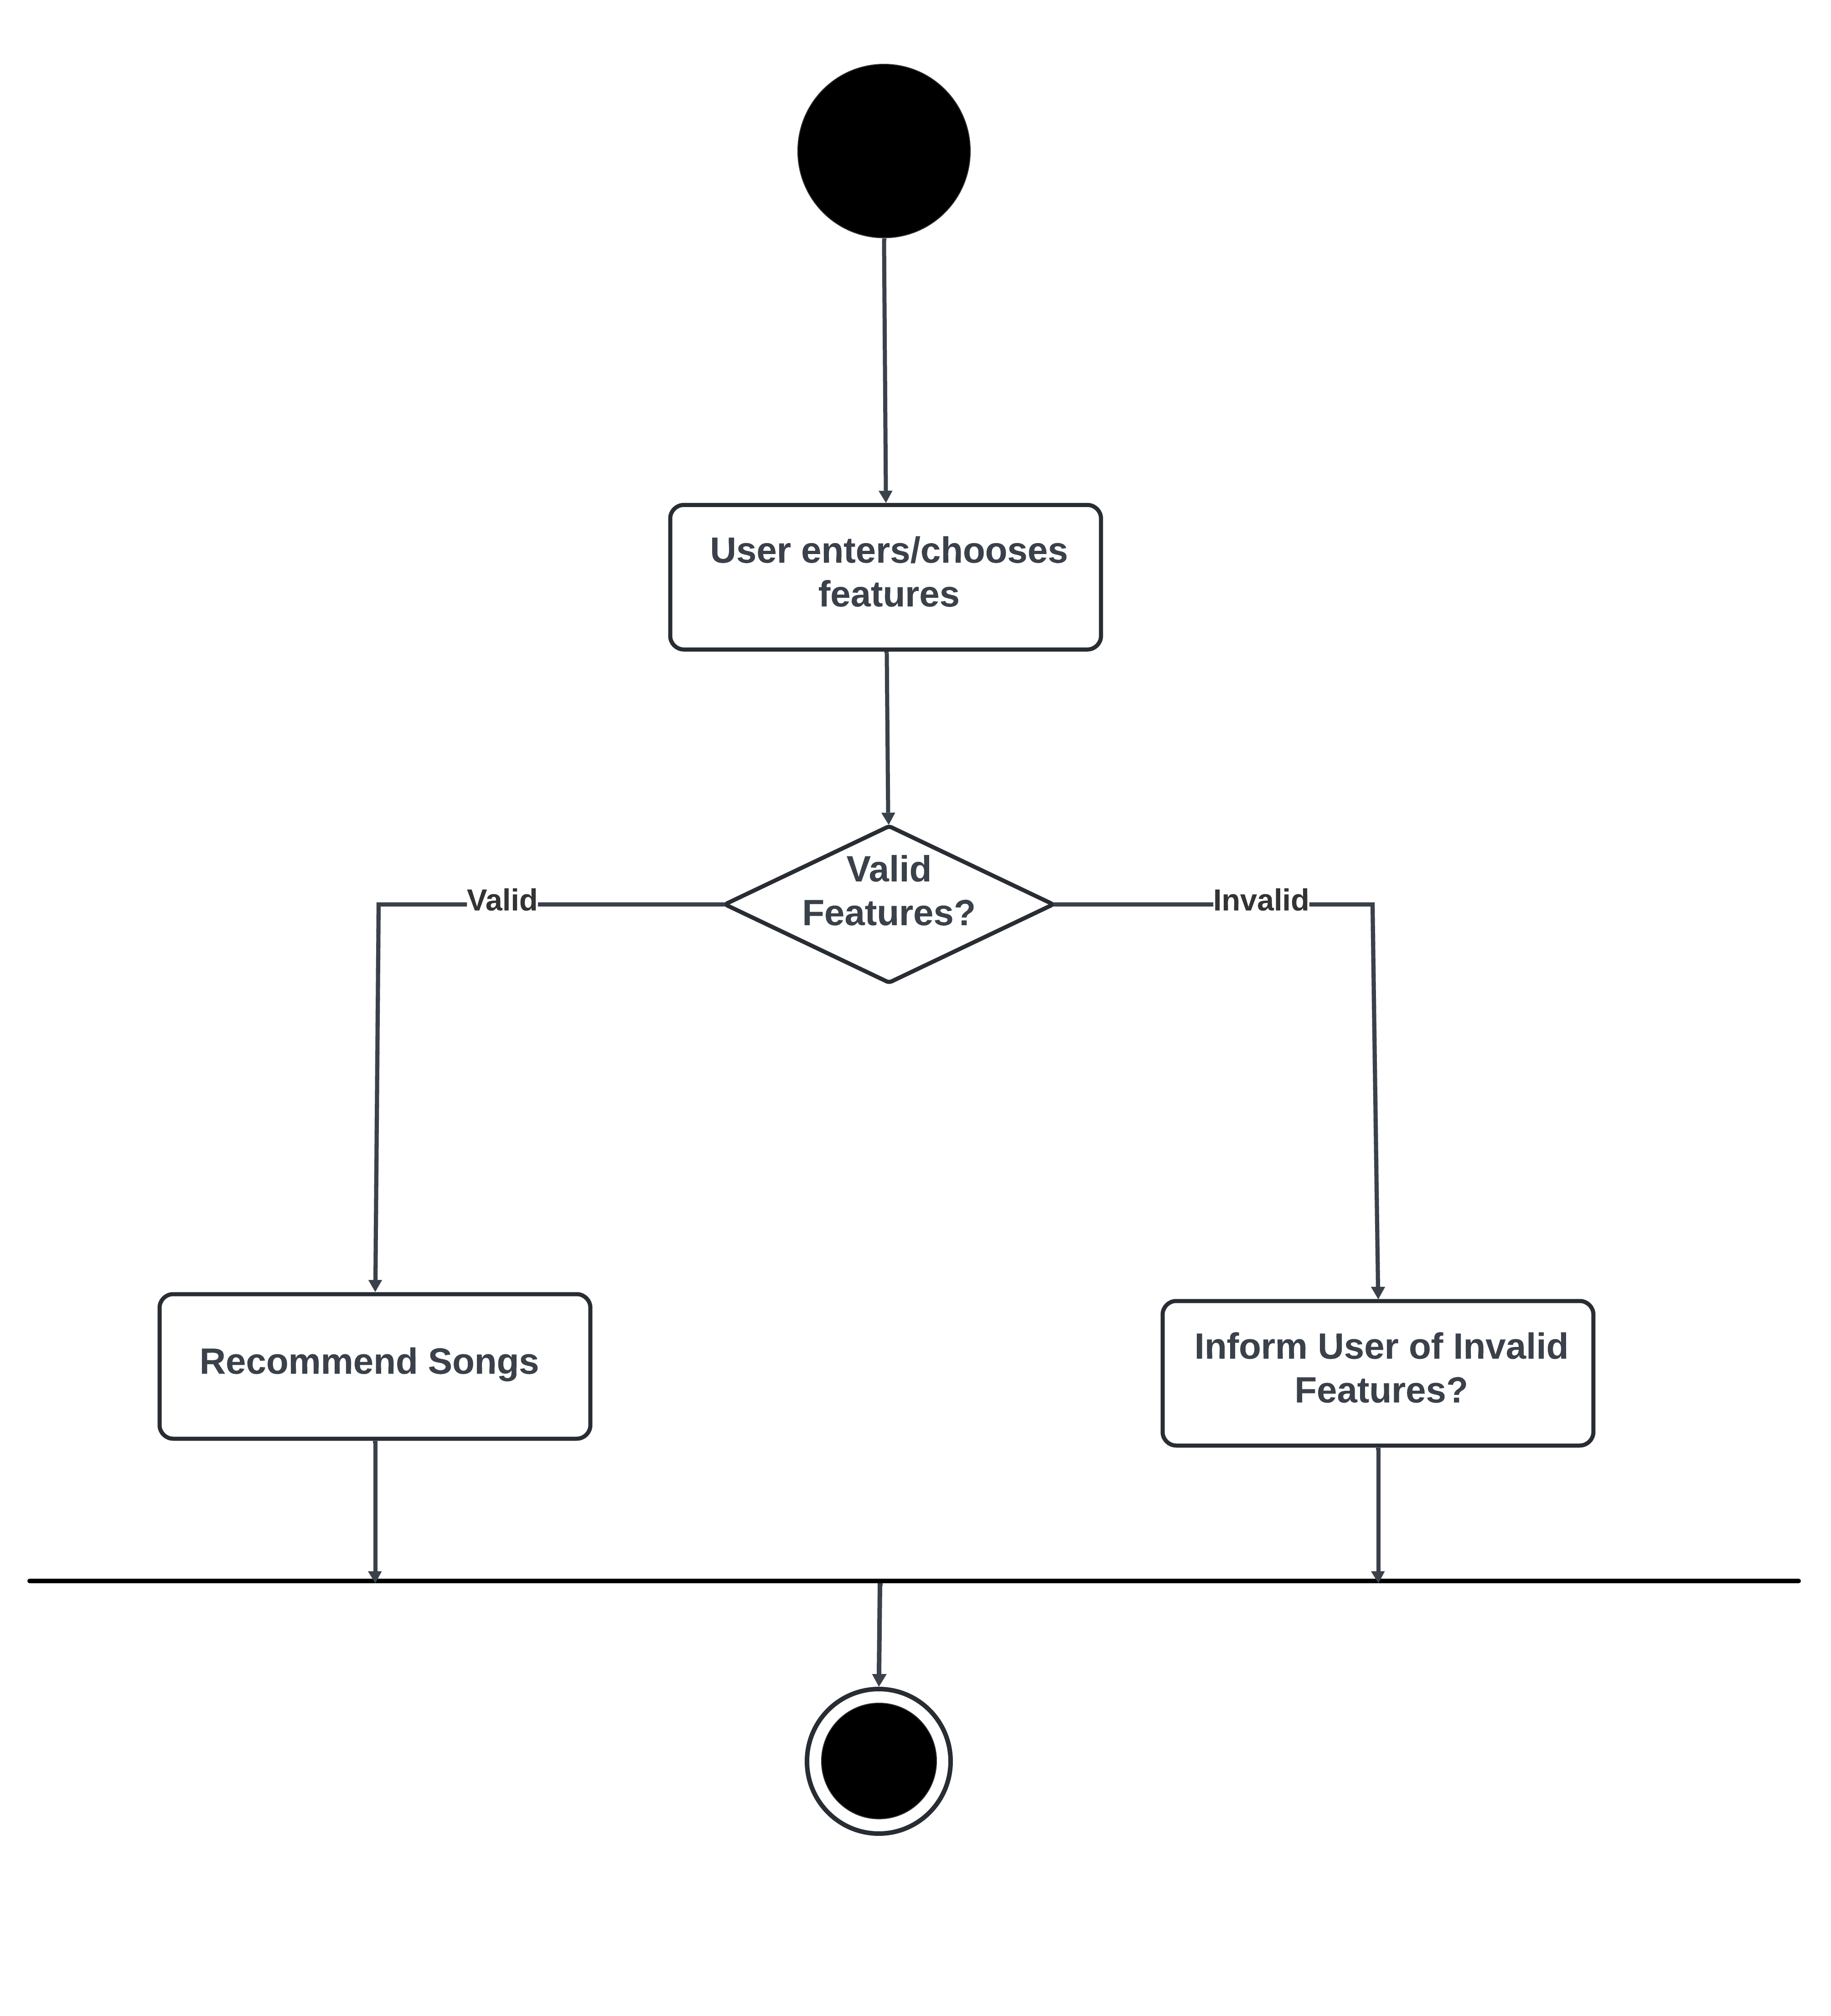
\includegraphics[width=\textwidth]{recommendation_feature.png} \\
\textbf{Outcome:} The user will select or manually enter features they are looking for in a song, and the system will first check to see if the features they selected/entered are valid, and the system will return a collection of reference songs that match those features.

\vspace{1cm}

\noindent \textbf{3. Product Use Case Name:} Music Generation Based on Input \\
\textbf{Trigger:} User inputs reference song(s) and/or song snippet(s), and indicates they want to generate a song \\
\textbf{Preconditions:} User must have GenreGuru open, and the user has provided a valid input(s) \\
\textbf{Interested Stakeholders:} Music producers, Hobbyist Musicians \\
\textbf{Actor/s:} User \\
\textbf{Activity Diagram:} \\
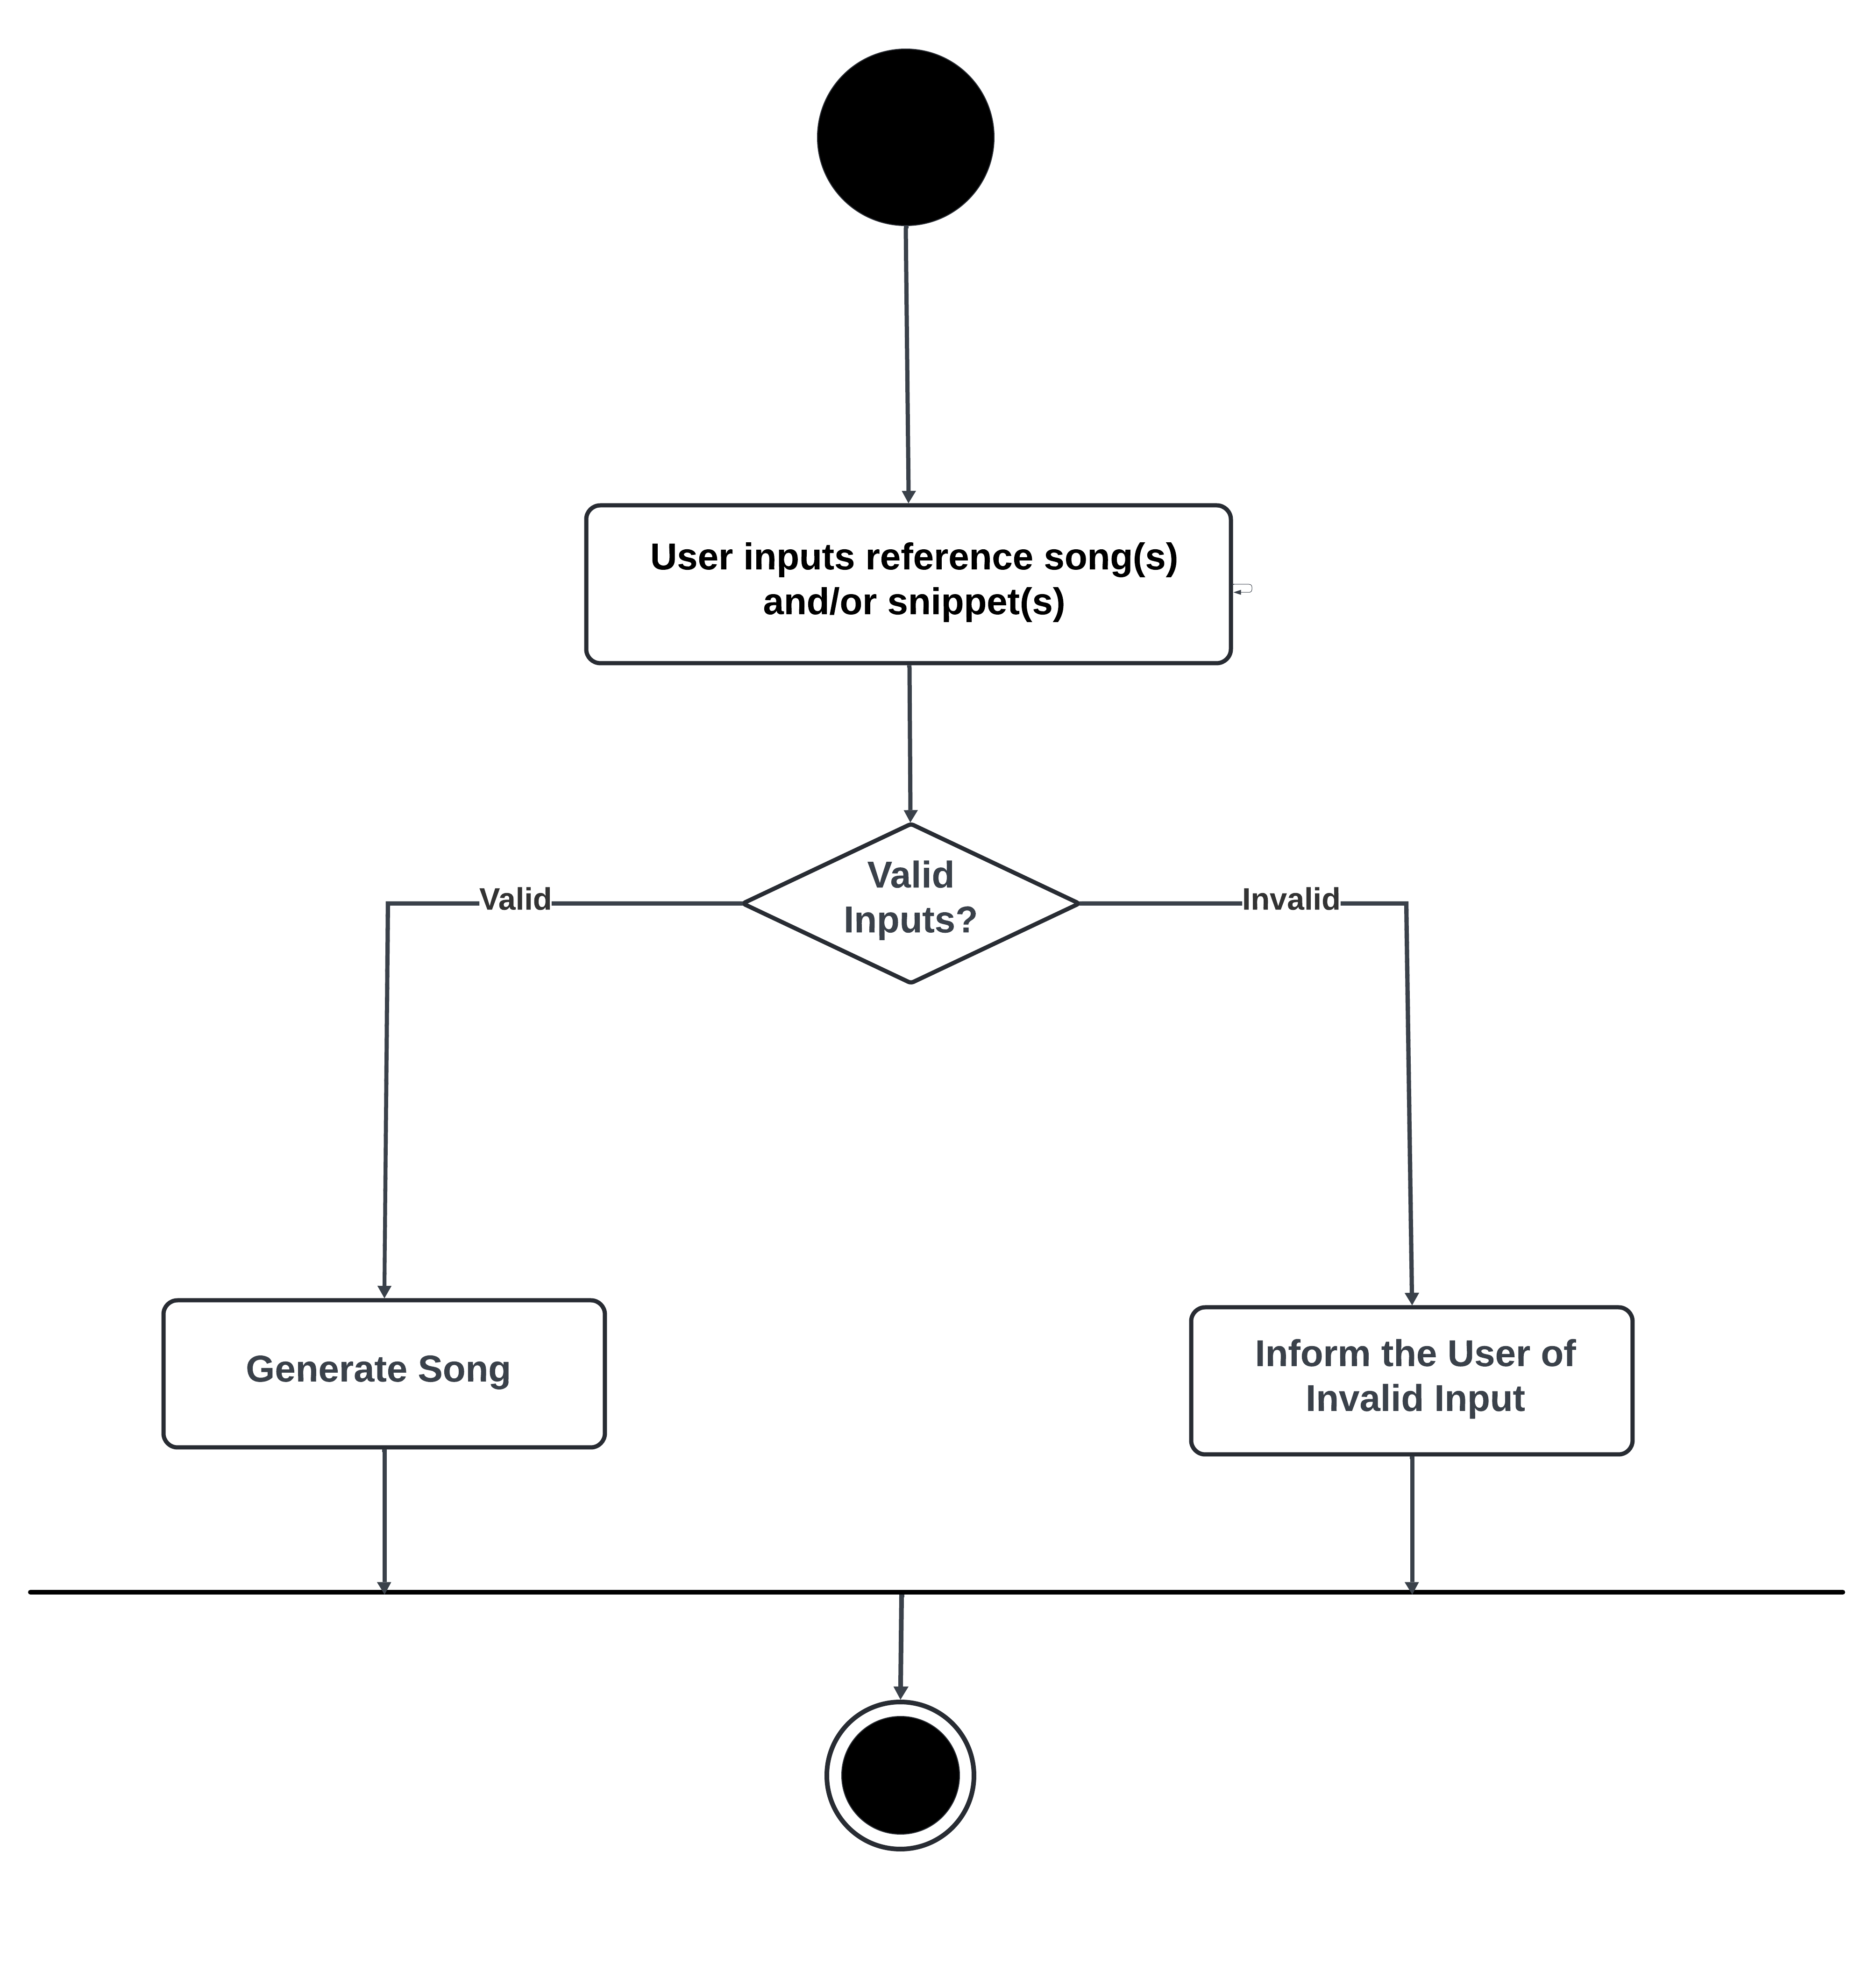
\includegraphics[width=\textwidth]{generate_song.png} \\
\textbf{Outcome:} The user will enter song(s) and/or song snippet(s) and indicate to the system that they want to generate music, the system will check that these inputs are valid (correct format) and then will generate a song and return it to the user.

\vspace{1cm}

\noindent \textbf{4. Product Use Case Name:} Analyze Music \\
\textbf{Trigger:} User inputs a reference song or song snippet and indicates they want to analyze the music \\
\textbf{Preconditions:} User must have GenreGuru open, and the user has provided a valid input \\
\textbf{Interested Stakeholders:} Music Producers, Audio Engineers, Music Educators \\
\textbf{Actor/s:} User \\
\textbf{Activity Diagram:} \\
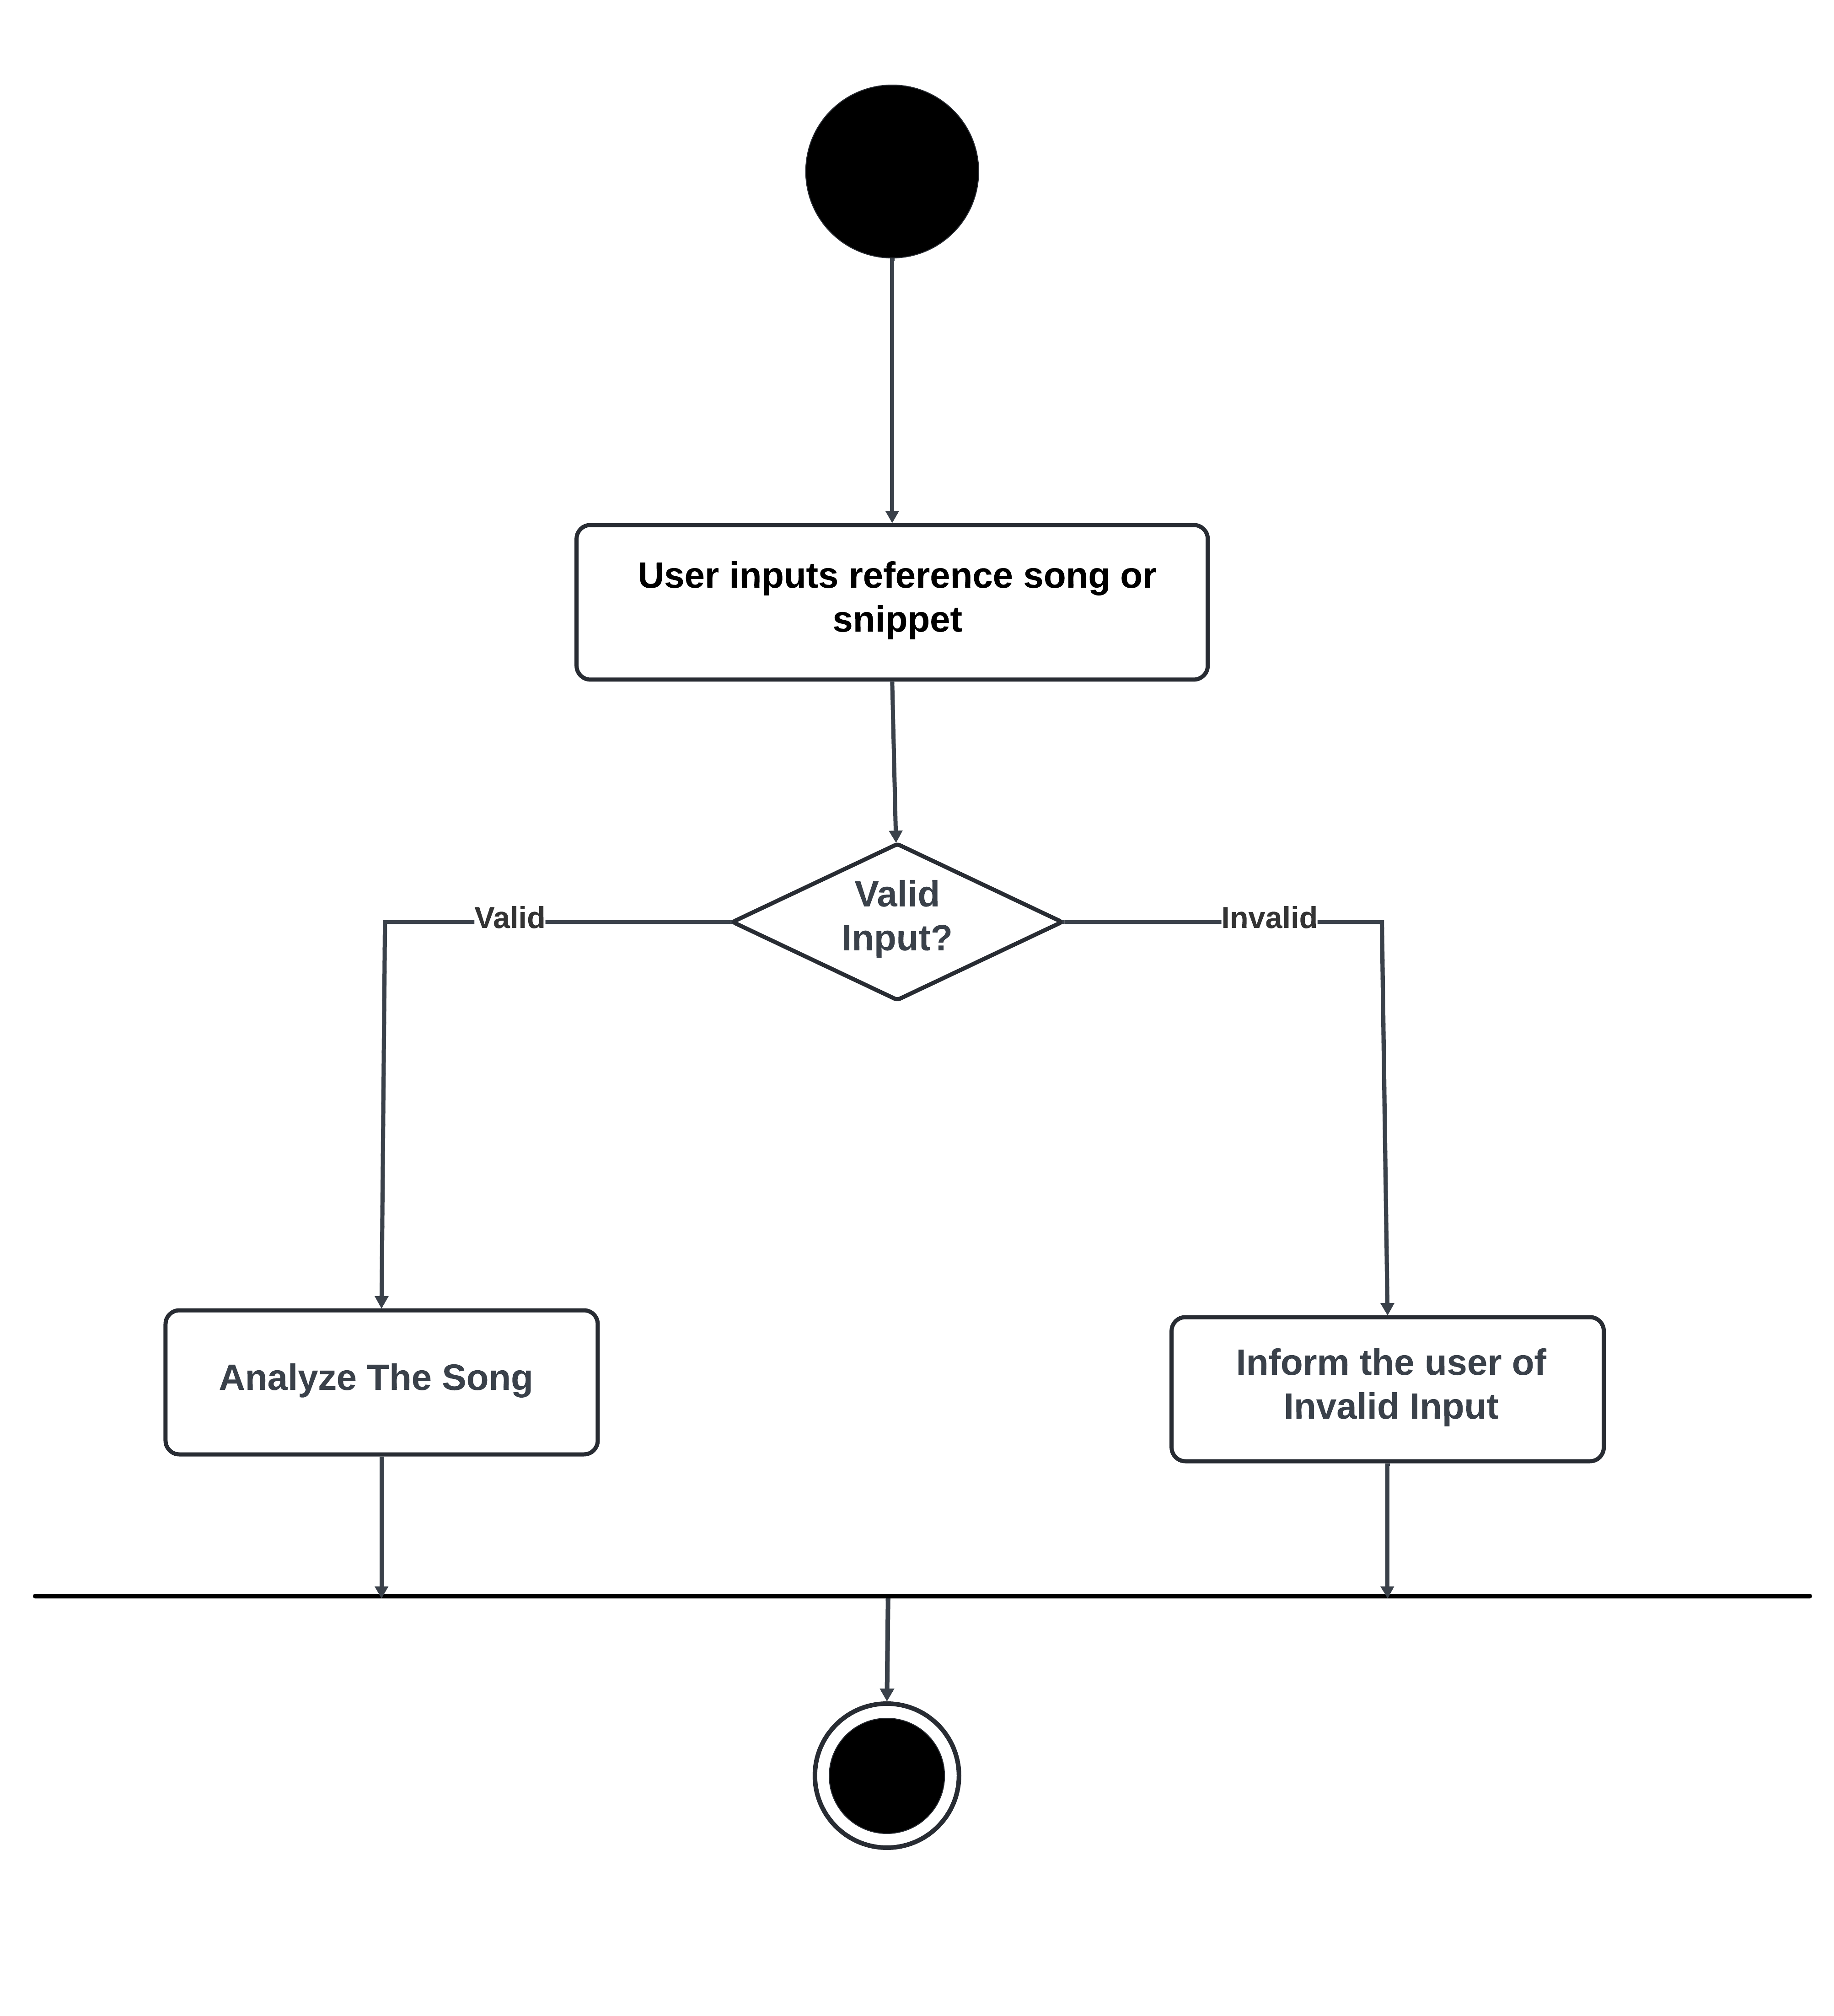
\includegraphics[width=\textwidth]{analyze_song.png} \\
\textbf{Outcome:} The user will input a reference song or song snippet and indicate they want to analyze the song, the system will validate the input and return a set of features and visualizations.

\vspace{1cm}

\noindent \textbf{5. Product Use Case Name:} Song Recommendation Based on Input \\
\textbf{Trigger:} User inputs reference song(s) and/or snippet(s), and indicates they want to search for recommendations \\
\textbf{Preconditions:} User must have GenreGuru open, and the user has provided a valid input(s) \\
\textbf{Interested Stakeholders:} Casual Music Listeners, Hobbyist Musicians \\
\textbf{Actor/s:} User \\
\textbf{Activity Diagram:} \\
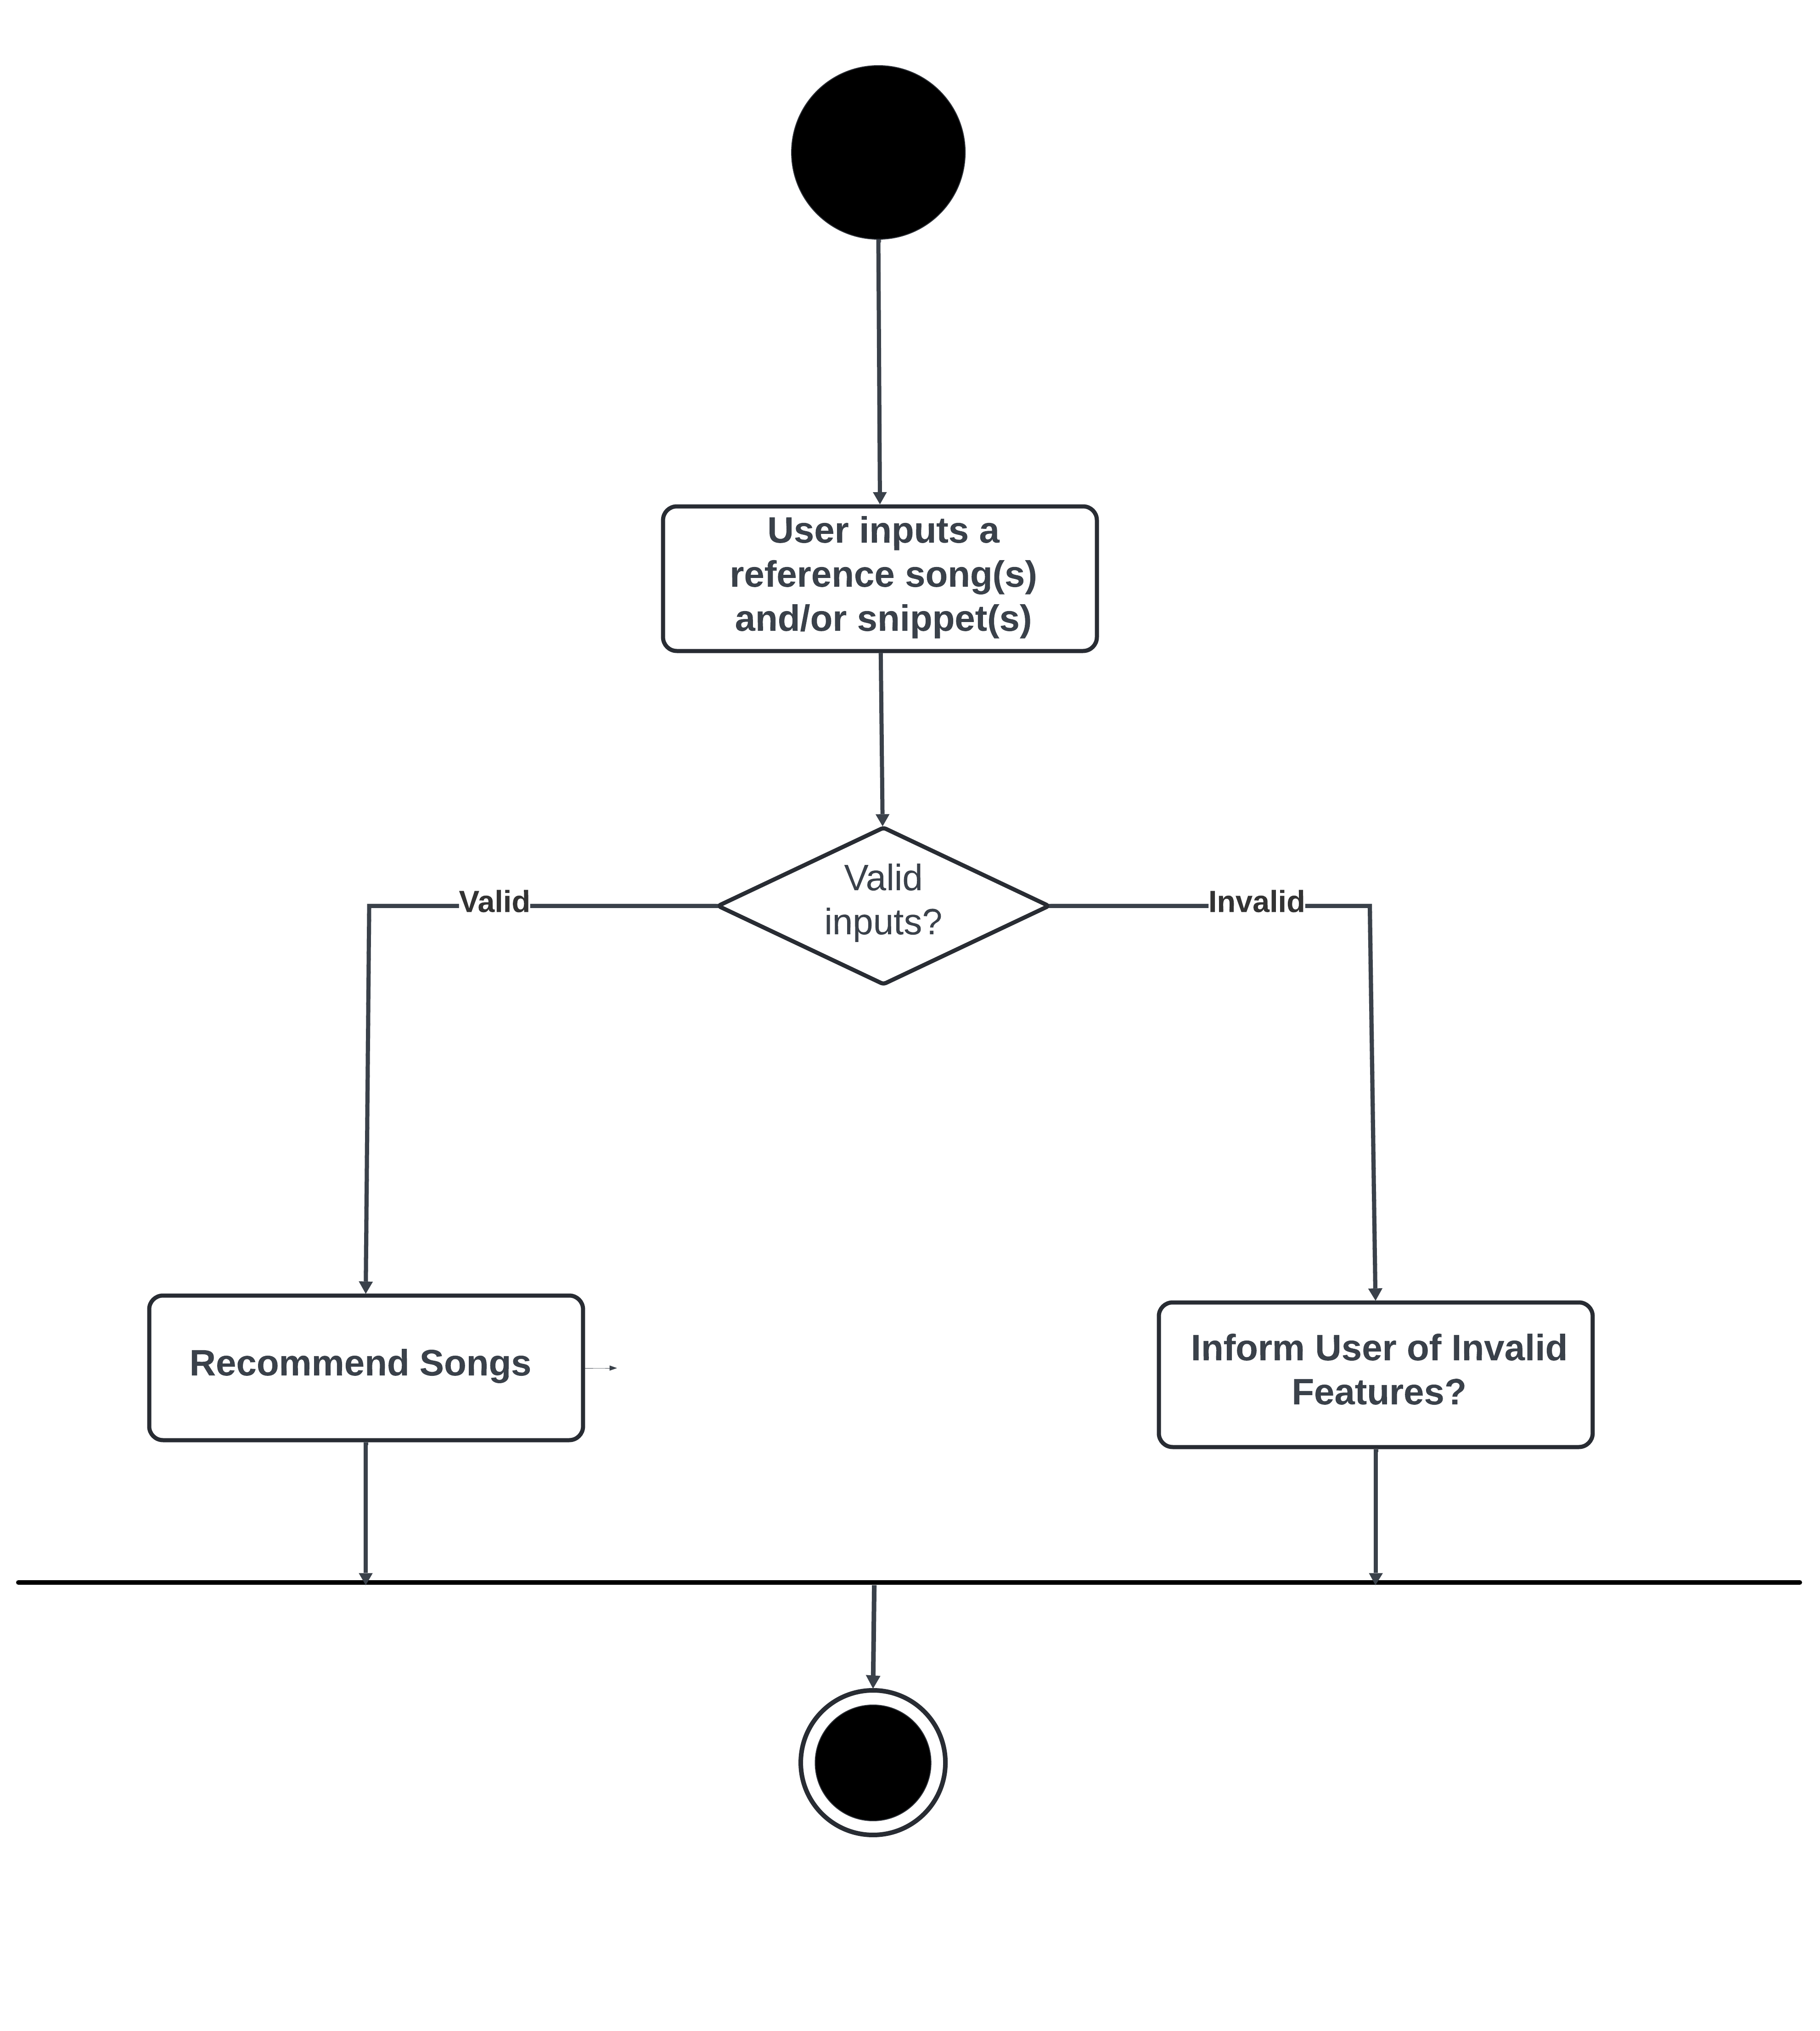
\includegraphics[width=\textwidth]{recommend_song.png} \\
\textbf{Outcome:} The users will input reference song(s) and/or snippet(s), the system will first check to see if the inputs are valid. Then the system will return a collection of reference songs.

\vspace{1cm}

\textbf{6. Product Use Case Name:} Server Interaction for Music Generation \\
\textbf{Trigger:} User submits a reference song and/or snippet and requests music generation \\
\textbf{Preconditions:} User has provided a valid input through, and the server is operational \\
\textbf{Interested Stakeholders:} Music Producers, Hobbyist Musicians \\
\textbf{Actor/s:} Server \\
\textbf{Activity Diagram:} \\
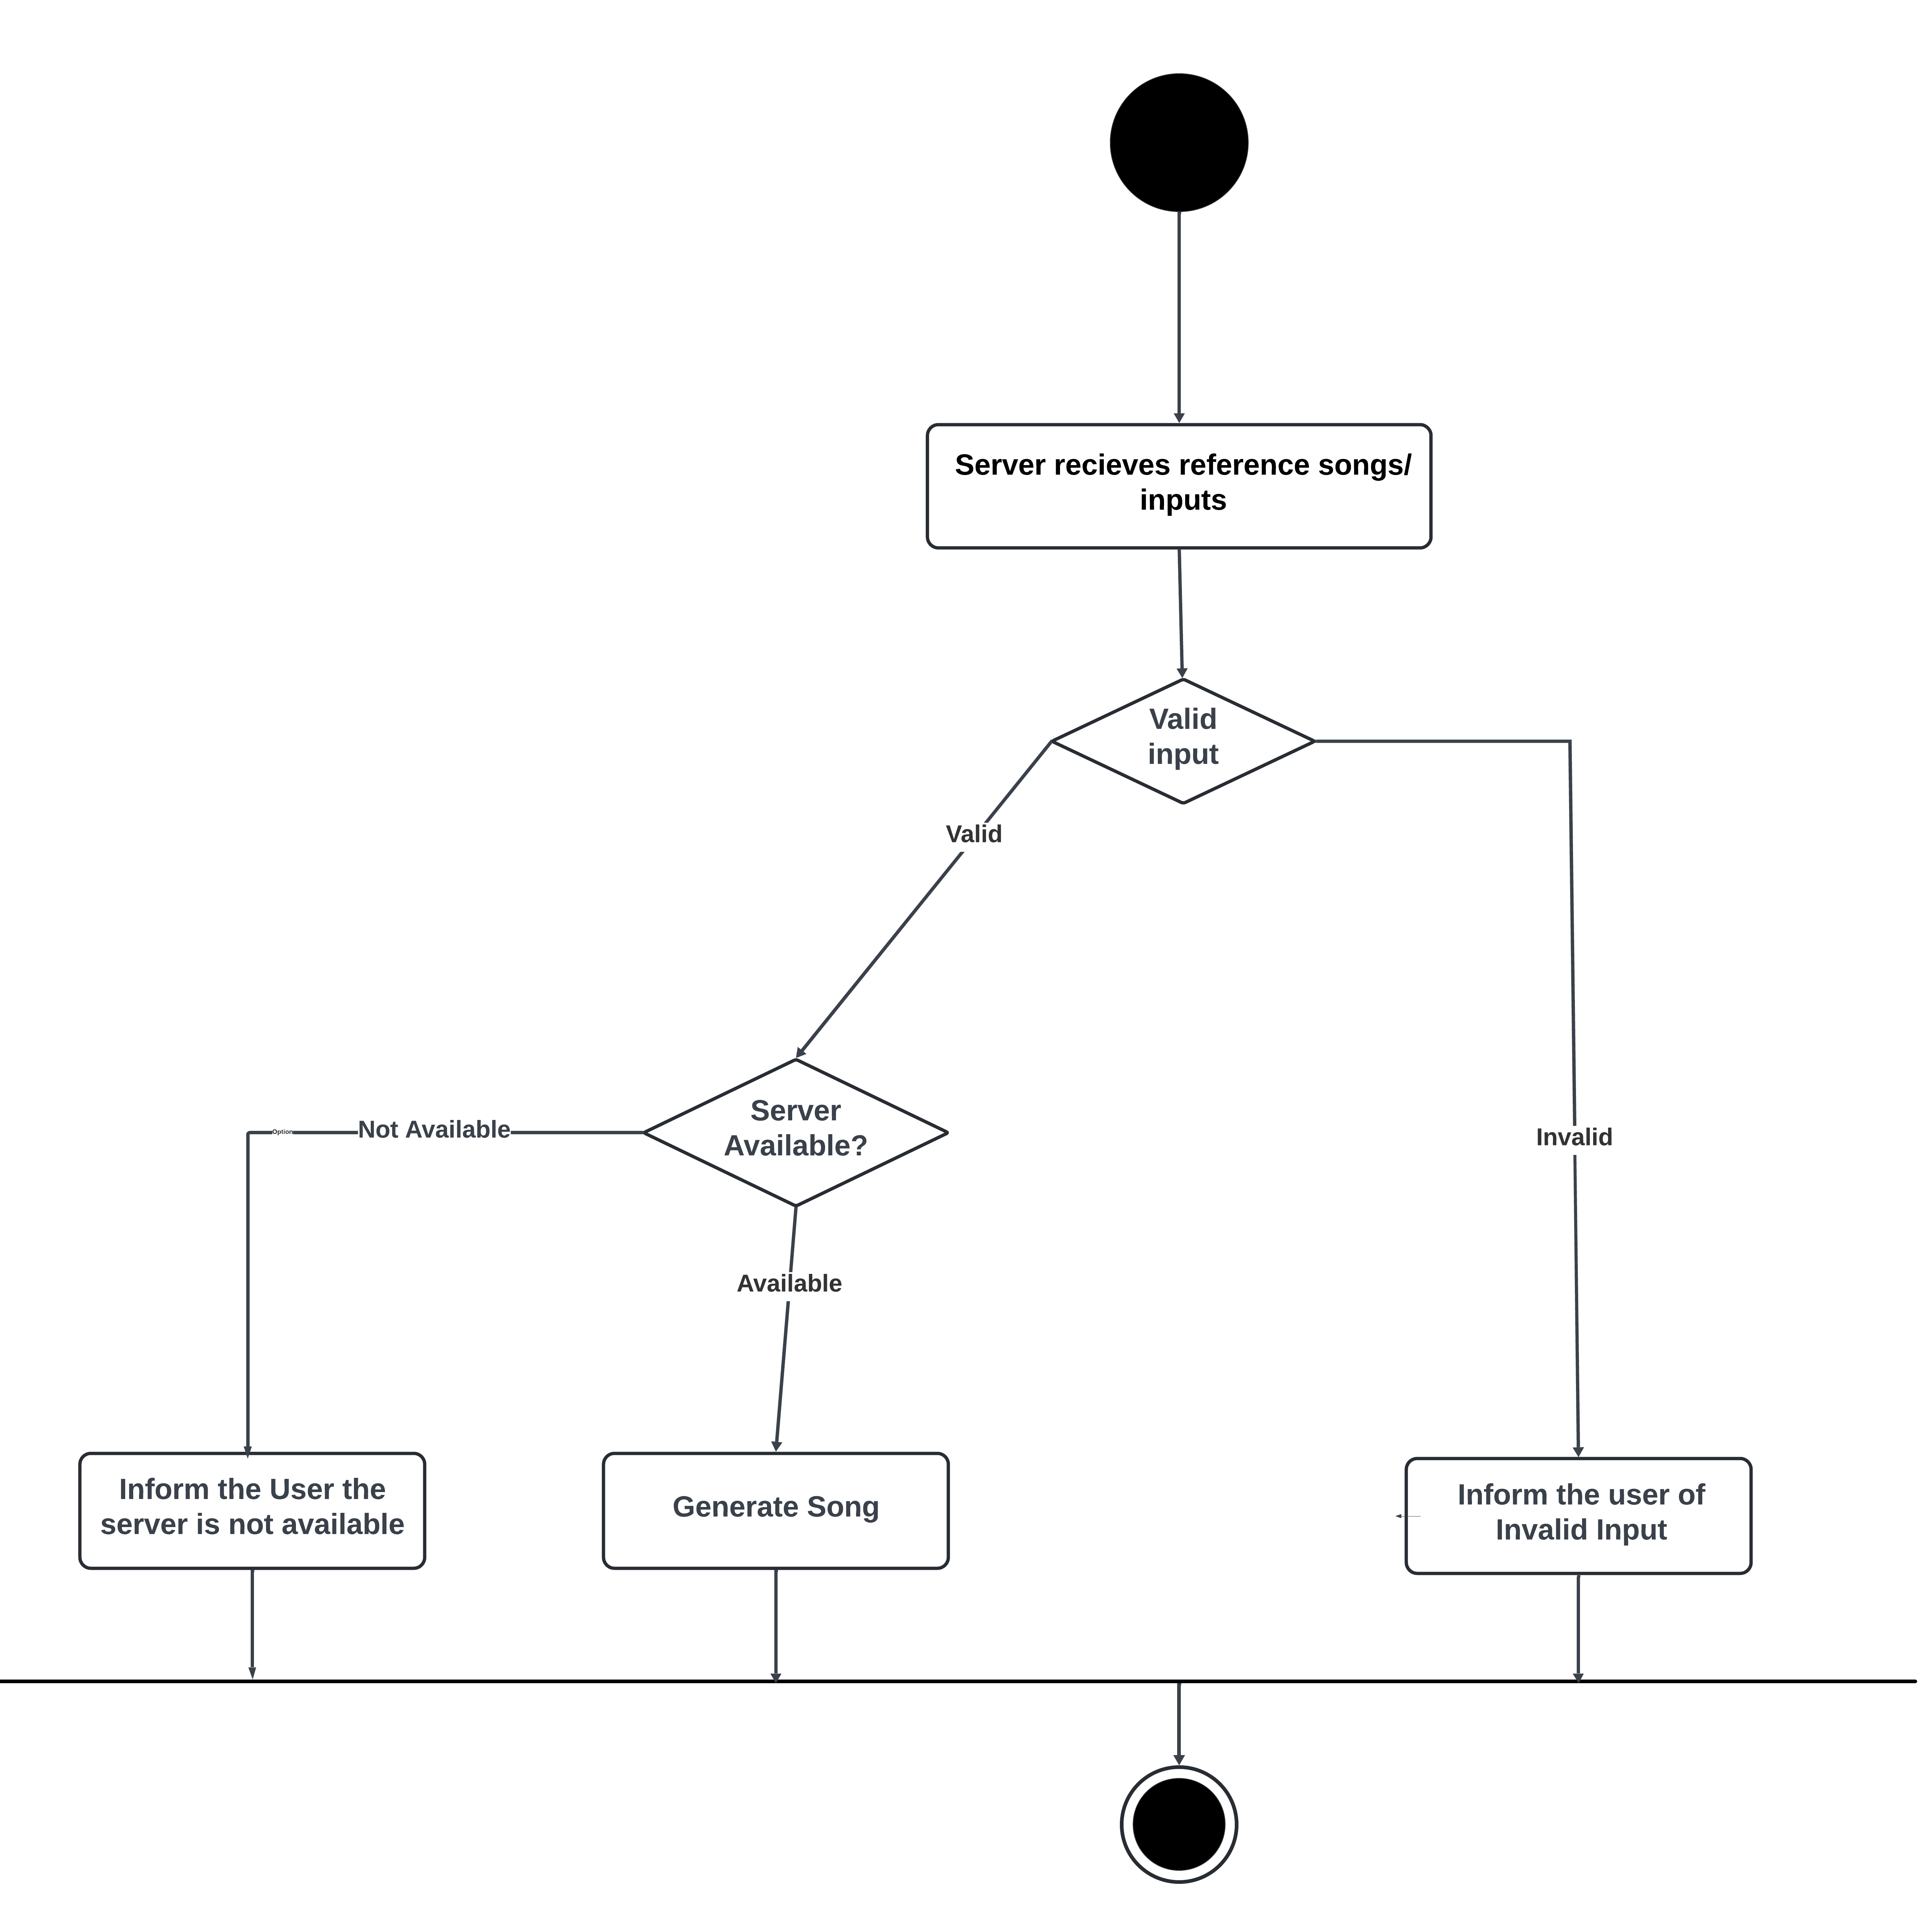
\includegraphics[width=\textwidth]{server_song_gen.png} \\
\textbf{Outcome:} The server processes the input, generates music, and returns the generated song to the user

\vspace{1cm}

\textbf{7. Product Use Case Name:} Server Interaction for Song Recommendation \\
\textbf{Trigger:} User submits desired features or reference songs/snippets and requests song recommendations \\
\textbf{Preconditions:} User has provided valid input, and the server is available \\
\textbf{Interested Stakeholders:} Casual Music Listeners, Hobbyist Musicians \\
\textbf{Actor/s:} Server \\
\textbf{Activity Diagram:} \\
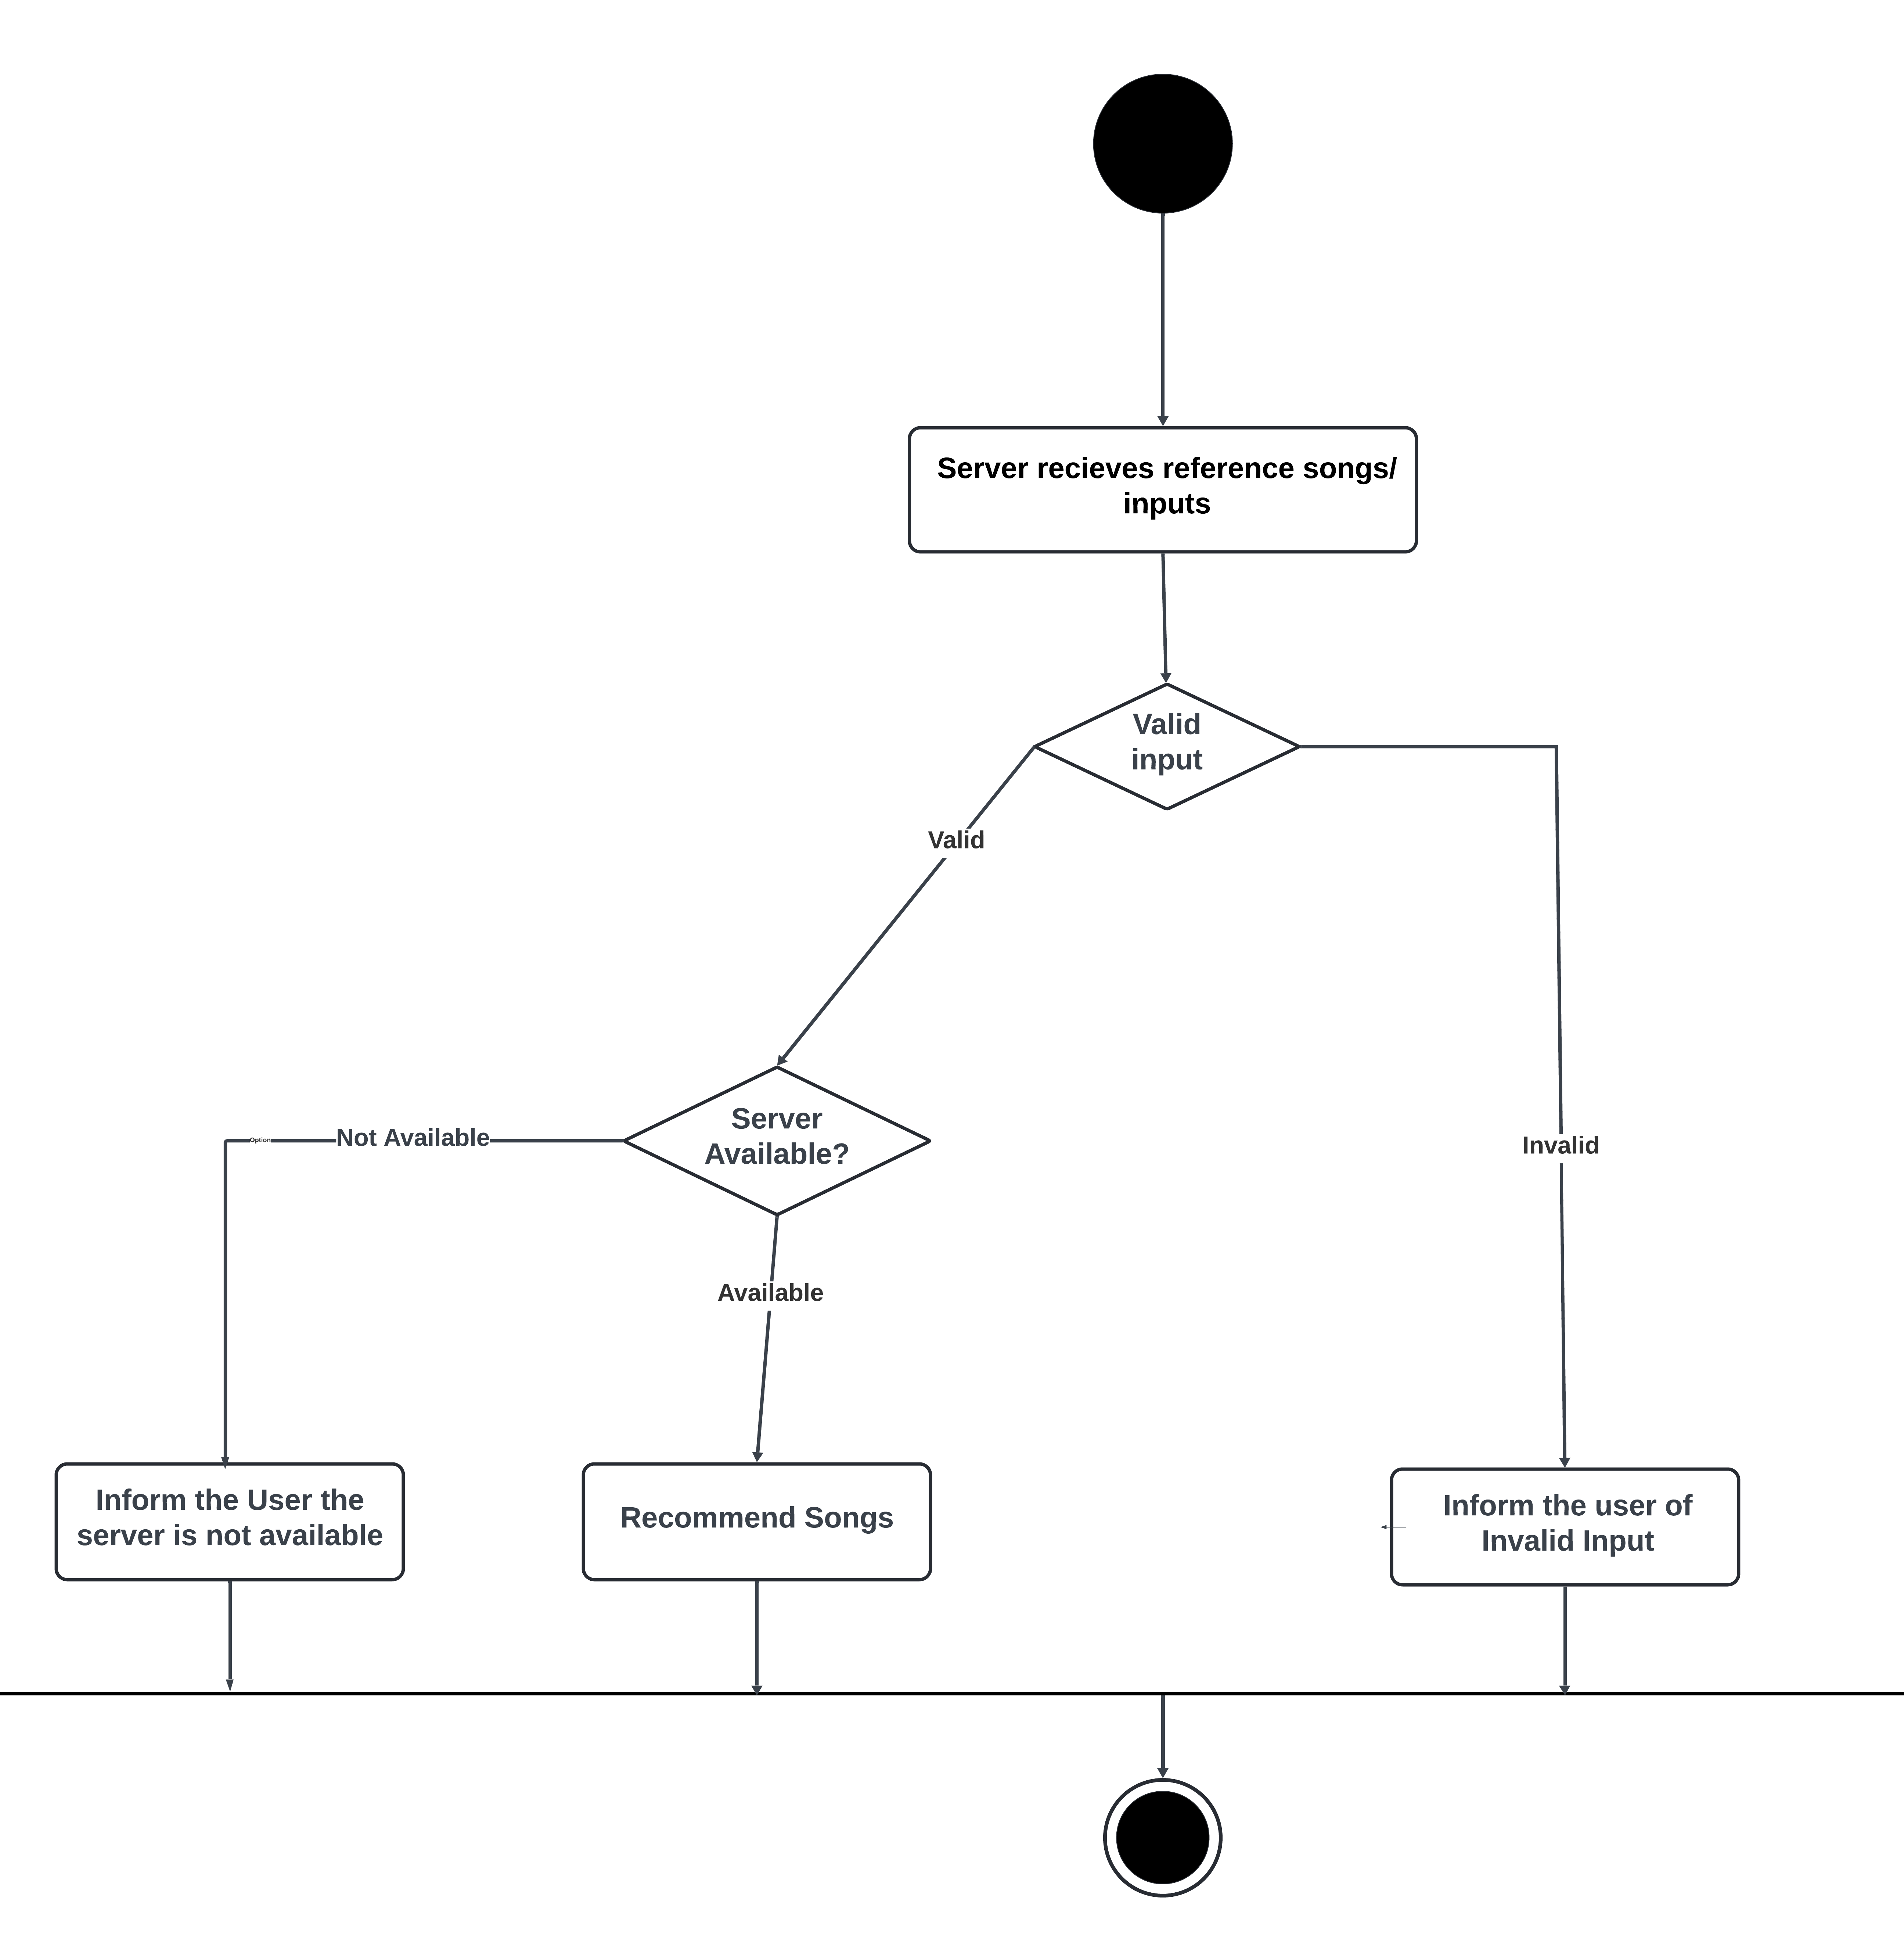
\includegraphics[width=\textwidth]{server_song_rec.png} \\
\textbf{Outcome:} The server processes the input and returns a collection of recommended songs based on the input features or reference songs/snippets.

\vspace{1cm}

\textbf{8. Product Use Case Name:} Server Interaction for Music Analysis \\
\textbf{Trigger:} User submits a reference song or snippet and requests music analysis \\
\textbf{Preconditions:} User has provided a valid input, and the server is ready to analyze \\
\textbf{Interested Stakeholders:} Music Producers, Audio Engineers, Music Educators \\
\textbf{Actor/s:} Server \ \textbf{Activity Diagram:} \\
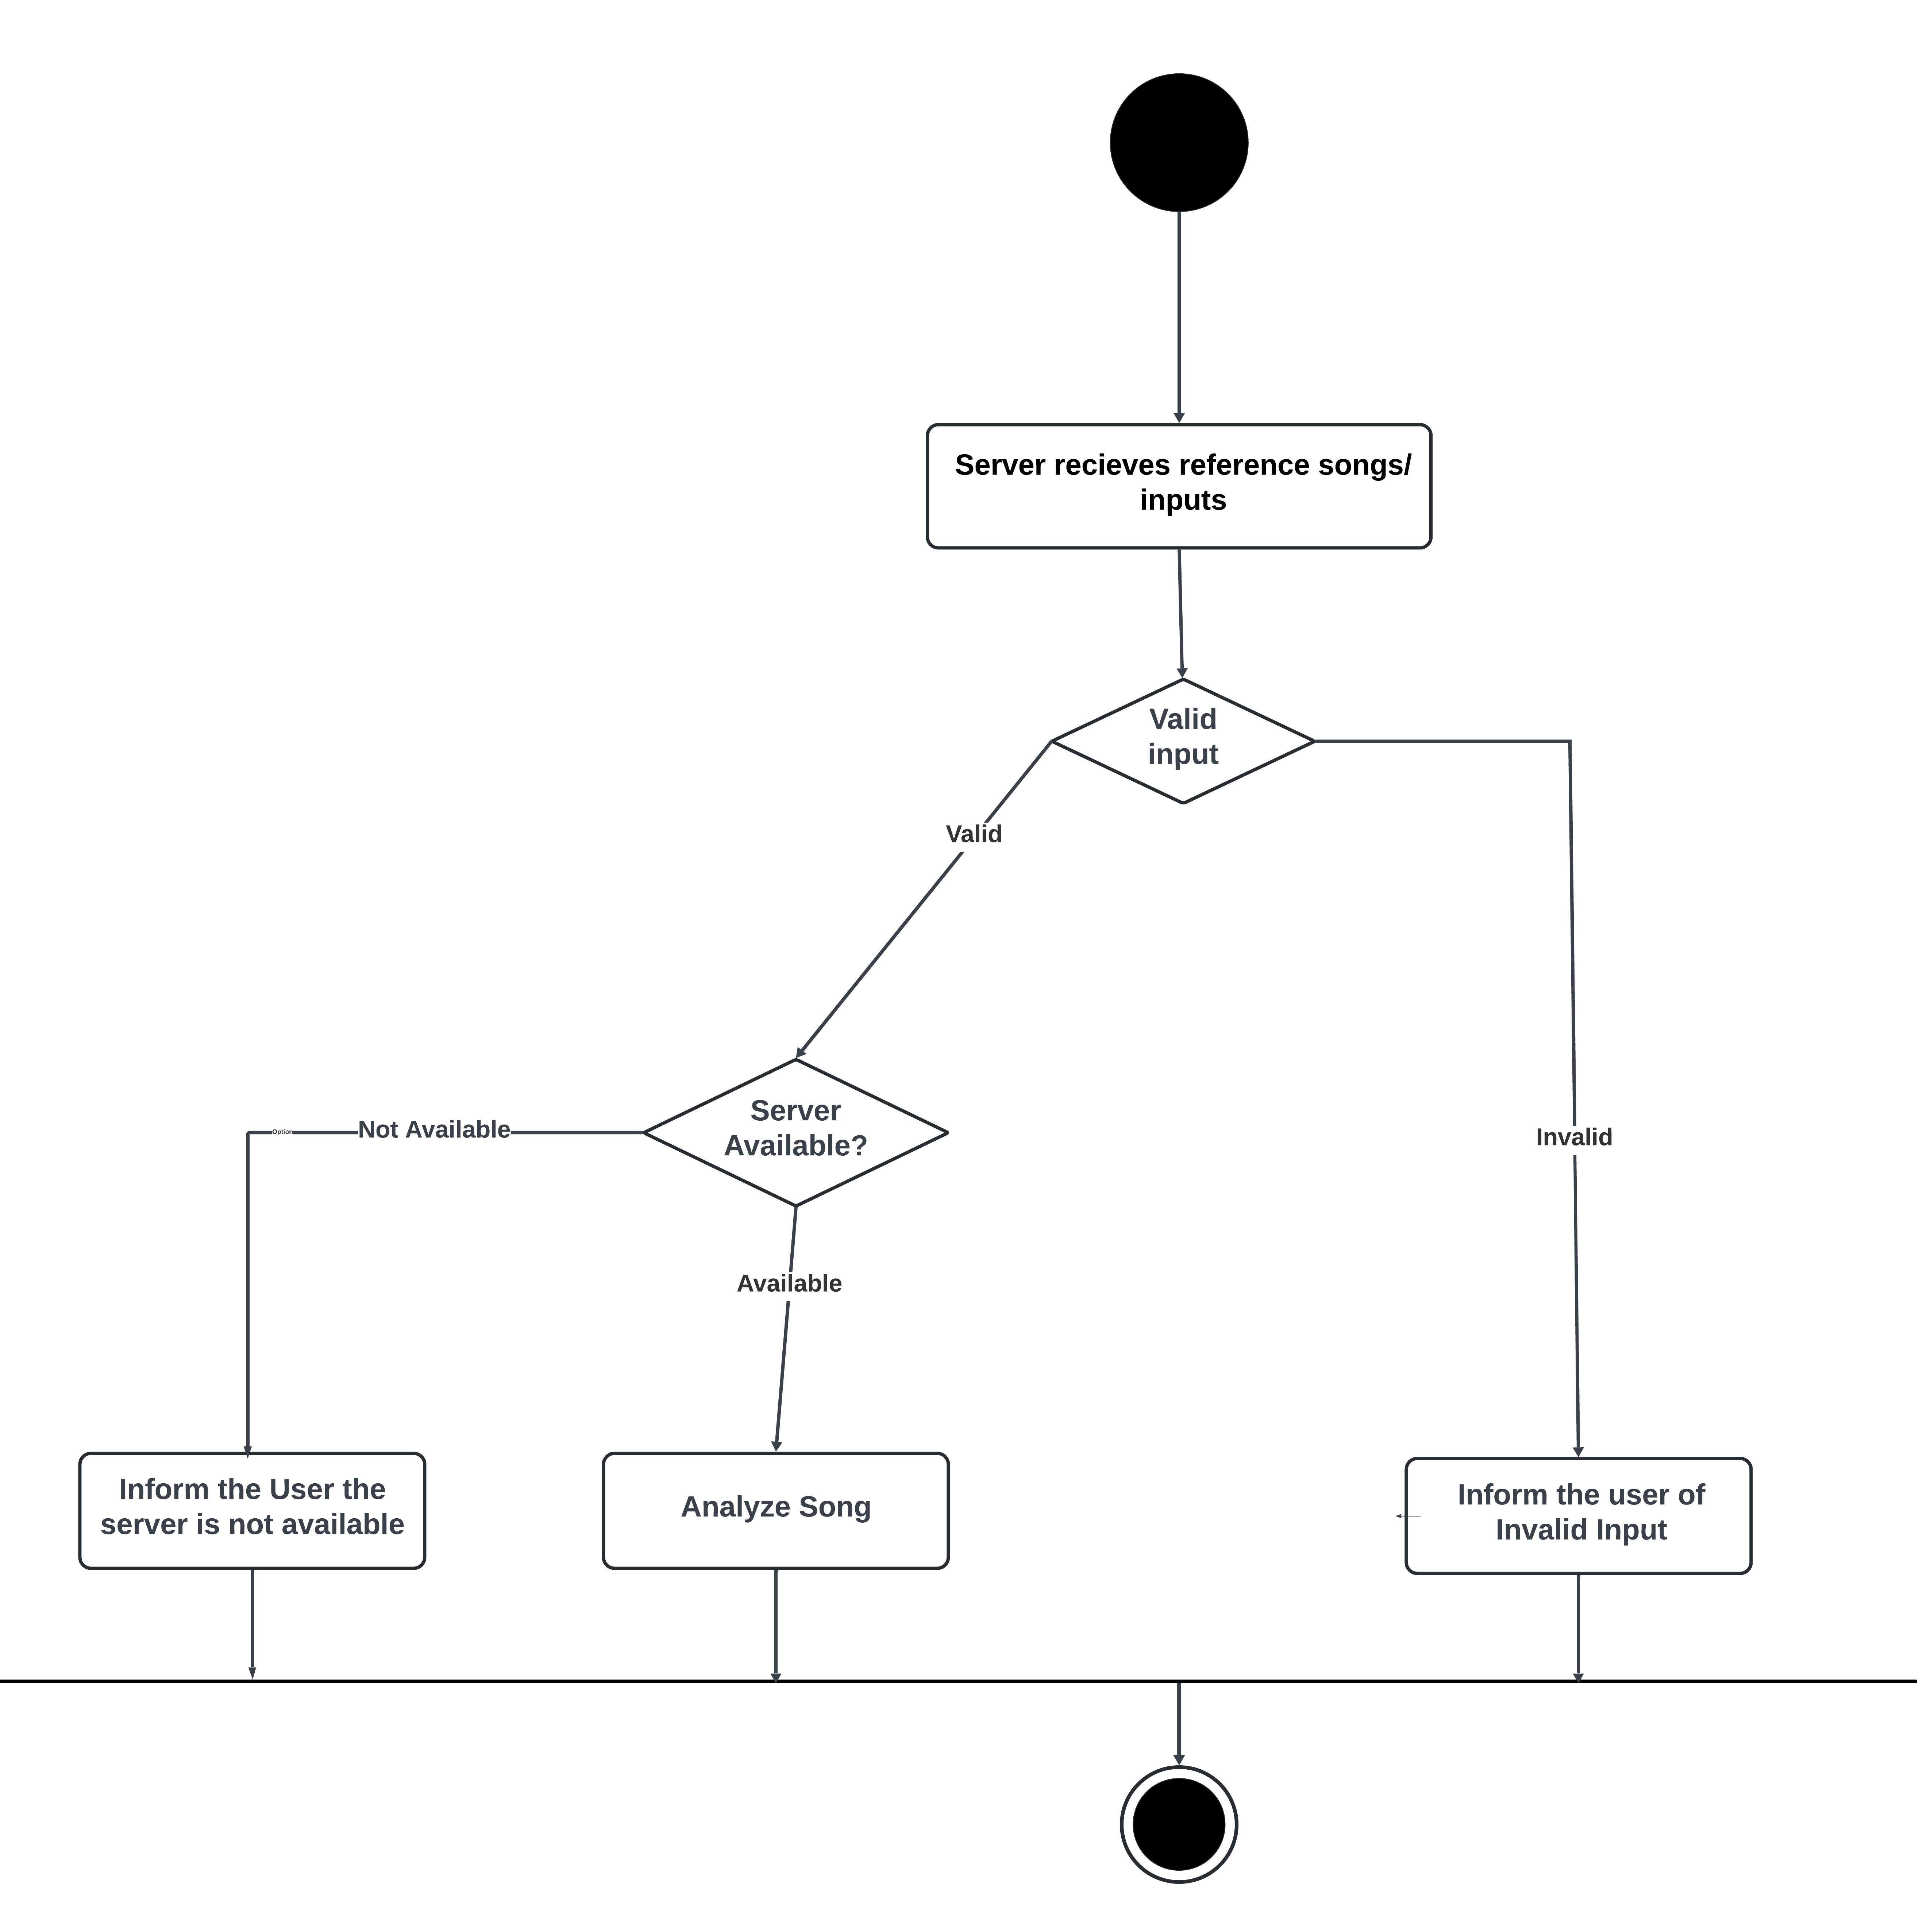
\includegraphics[width=\textwidth]{server_song_analysis.png} \\
\textbf{Outcome:} The server analyzes the song or snippet and returns a collection of features and visualizations to the user.

\section{Functional Requirements}
\subsection{Functional Requirements}
\lips

\section{Look and Feel Requirements}
\subsection{Appearance Requirements}
\lips
\subsection{Style Requirements}
\lips

\section{Usability and Humanity Requirements}
\subsection{Ease of Use Requirements}
\lips
\subsection{Personalization and Internationalization Requirements}
\lips
\subsection{Learning Requirements}
\lips
\subsection{Understandability and Politeness Requirements}
\lips
\subsection{Accessibility Requirements}
\lips

\section{Performance Requirements}
\subsection{Speed and Latency Requirements}
\lips
\subsection{Safety-Critical Requirements}
\lips
\subsection{Precision or Accuracy Requirements}
\lips
\subsection{Robustness or Fault-Tolerance Requirements}
\lips
\subsection{Capacity Requirements}
\lips
\subsection{Scalability or Extensibility Requirements}
\lips
\subsection{Longevity Requirements}
\lips

\section{Operational and Environmental Requirements}
\subsection{Expected Physical Environment}
\lips
\subsection{Wider Environment Requirements}
\lips
\subsection{Requirements for Interfacing with Adjacent Systems}
\lips
\subsection{Productization Requirements}
\lips
\subsection{Release Requirements}
\lips

\section{Maintainability and Support Requirements}
\subsection{Maintenance Requirements}
\lips
\subsection{Supportability Requirements}
\lips
\subsection{Adaptability Requirements}
\lips

\section{Security Requirements}
\subsection{Access Requirements}
\lips
\subsection{Integrity Requirements}
\lips
\subsection{Privacy Requirements}
\lips
\subsection{Audit Requirements}
\lips
\subsection{Immunity Requirements}
\lips

\section{Cultural Requirements}
\subsection{Cultural Requirements}
\lips

\section{Compliance Requirements}
\subsection{Legal Requirements}
\lips
\subsection{Standards Compliance Requirements}
\lips

\section{Open Issues}
\lips

\section{Off-the-Shelf Solutions}
\subsection{Ready-Made Products}
\lips
\subsection{Reusable Components}
\lips
\subsection{Products That Can Be Copied}
\lips

\section{New Problems}

\subsection{Effects on the Current Environment}

The platform's high computational requirements, especially during the training and usage of generative models, may put a strain on existing computational resources. This could lead to slower performance for other applications that share these resources. Additionally, increased data transmission due to the integration with APIs such as Spotify and Deezer could lead to higher network bandwidth utilization, potentially affecting the performance of other network-dependent systems. Mitigating these effects may require infrastructure scaling, such as increasing server capacity or optimizing data processing, to ensure that the existing systems are not disrupted.

\subsection{Effects on the Installed Systems}

The new platform will interact with various installed systems, leading to the introduction of new dependencies. For example, using third-party APIs like Spotify or integrating machine learning frameworks such as TensorFlow may require changes to the current software stack. These dependencies could introduce compatibility issues, particularly if third-party providers update their APIs or if new versions of required libraries are released. Such updates might necessitate timely system changes to maintain functionality and avoid disruptions. Ensuring that installed systems remain compatible requires diligent version management, comprehensive testing, and a structured process for managing library and API updates.

\subsection{Potential User Problems}

The platform is designed to offer advanced features, which may present usability challenges for some users. For example, users with limited technical skills may struggle to understand the process of modifying musical features like key, rhythm, or tempo, which are essential for customizing music generation. Furthermore, the quality of generated outputs is inherently subjective, and users may feel frustrated if the system-generated music does not meet their expectations. Another potential problem is system latency, especially when resource-intensive operations like model inference are being performed. Long waiting times could negatively impact user experience, making the platform feel less responsive, which may deter regular use.

\subsection{Limitations in the Anticipated Implementation Environment That May Inhibit the New Product}

The platform is expected to be implemented on a local server, which presents certain limitations. The local server environment will need sufficient processing power to handle computationally intensive tasks, such as model training and music generation. If the server infrastructure is under-resourced, performance issues such as latency and reduced processing speed could arise. Additionally, reliance on a local server means that the platform's effectiveness is tied directly to server availability and maintenance. Any server downtime could render the platform inaccessible to users. If we decide to extend the platform's implementation onto personal devices, new limitations arise. Personal devices, especially those with limited hardware capabilities, may struggle with the computational requirements of generative music models, leading to significant performance bottlenecks. This could make the platform inaccessible or difficult to use for some users. Moreover, the reliance on internet connectivity for accessing external APIs is another major limitation. Users in areas with unreliable internet or low bandwidth may face difficulties, particularly with real-time features like music recommendations or generating new songs based on streaming data. These limitations could restrict the user base to only those with high-performance devices and stable internet connections.

\subsection{Follow-Up Problems}

Once the platform is deployed, several follow-up issues will need to be addressed to maintain and improve the product. One of the primary challenges will be keeping up with third-party API changes, such as modifications to Spotify or Deezer APIs, which could lead to broken features if not handled promptly. The generative models used by the platform will also require regular updates and retraining to stay relevant to emerging musical styles and user preferences. Another follow-up problem is related to usability: feedback from users might reveal unforeseen pain points or desired improvements. Addressing these concerns will require an iterative development approach, incorporating user feedback into future versions of the platform to enhance usability and performance.


\lips
\subsection{Follow-Up Problems}
\lips

\section{Tasks}
\subsection{Project Planning}
\lips
\subsection{Planning of the Development Phases}
\lips

\section{Migration to the New Product}
\subsection{Requirements for Migration to the New Product}
There are no migration requirements as this project is not a replacement or upgrade of a previous project
\subsection{Data That Has to be Modified or Translated for the New System}
Similarly, there currently is no data that needs to be modified

\section{Costs}
The monetary cost estimate of the project is \$0 CAD. All of the necessary equipment is
owned by at least one group member.\\

\noindent
The total time cost estimate of the project is 8 months (September 2024 - April 2025).\\

\noindent
The function point cost estimate is 12. This is derived from the above sections, mainly the functional
requirements, non-functional requirements, and business rules
\section{User Documentation and Training}

\subsection{User Documentation Requirements}

The music featurization feature is heavily API-driven, and as such, detailed documentation will primarily be covered within the API reference section. This approach ensures that developers and advanced users can understand the feature's capabilities without needing additional user guides.

To ensure that users can effectively interact with the music generation and recommendation platform, the following user documentation will be provided:

\begin{itemize}
  \item \textbf{Quick Start Guide}: A concise guide aimed at helping new users get started with the basics of generating and recommending music.
  \item \textbf{API Reference and Technical Specifications}: Detailed documentation of the platform’s API, including available endpoints, request/response formats, and example queries. This reference is crucial for developers and advanced users who want to integrate the platform with other applications or automate tasks.
  \item \textbf{Installation Guide}: A step-by-step guide for installing the platform on local servers, including system requirements, installation commands, and troubleshooting common setup issues.
  \item \textbf{FAQs and Troubleshooting}: A list of frequently asked questions and troubleshooting tips to help users solve common issues independently.
  \item \textbf{Video Tutorials}: Step-by-step video guides that visually demonstrate key features and workflows, including setting up the platform, using the API, and generating music.
\end{itemize}

These documents will be designed for users of varying technical backgrounds to ensure they can fully utilize the platform's capabilities. The documentation will be created and maintained primarily by the development team, ensuring accuracy and alignment with the latest platform features. However, feedback from user groups will be actively sought to improve clarity and address any documentation gaps. Updates to the API reference and technical specifications will be managed as part of the regular software update cycle.
\subsection{Training Requirements}

To provide users with sufficient knowledge to operate the platform effectively, the following training resources will be developed:

\begin{itemize}
  \item \textbf{Video Tutorials}: Developed by the development team, these tutorials will cover various aspects of the platform, including API usage, generating music, and using advanced features. 
  \item \textbf{Online Training Modules}: If additional resources become available, online training modules could be developed to provide users with a structured learning path. However, due to current resource constraints, we do not plan to offer live training sessions.
\end{itemize}

These training requirements aim to encourage users to explore the full potential of the platform, regardless of their prior experience in music production or technology.


\section{Waiting Room}
\begin{enumerate}
  \item The recommendation system will be able to recommend songs from less popular music genres (jazz, blues, etc.)
  \item The analysis system will be able to extract musical features from less popular music genres (jazz, blues, etc.)
  \item The generative system will be able to generate songs from less popular music genres (jazz, blues, etc.)
  \item The recommendation system will be able to recommend songs from unpopular music genres (gnawa, libyan funk, etc.)
  \item The analysis system will be able to extract musical features from less popular music genres (gnawa, libyan funk, etc.)
  \item The generative system will be able to generate songs from less popular music genres (gnawa, libyan funk, etc.)
  \item The recommendation system will be able to search for songs with cover art similar to an input song
  \item The generative system will be able to generate new cover art for a newly generated song, based on the user's
  input criteria
  \item The generative system will be able to generate new covert art for an existing song
\end{enumerate}

\section{Ideas for Solution}

\begin{itemize}
    \item \textbf{Hybrid Recommendation System}: 
    A hybrid recommendation system combines content-based filtering and collaborative filtering techniques to provide a more personalized experience for users. Content-based filtering analyzes song features, such as genre, key, and rhythm, to suggest similar tracks. Collaborative filtering uses user preferences and historical listening patterns to suggest music. By combining these approaches, the system can offer users personalized suggestions while also helping them discover new genres and music styles.

    \item \textbf{Generative Music Model}: 
    To enable the creation of new music, a generative model will be used. This model could be based on techniques such as a Generative Adversarial Network (GAN) or Recurrent Neural Network (RNN). A GAN would allow for the generation of realistic music by having the generator and discriminator work together to produce convincing compositions. An RNN, on the other hand, would be well-suited for learning the sequential nature of music, generating new melodies based on learned patterns. This solution provides users with an innovative way to create new music based on their inputs and preferences.

    \item \textbf{Feature Manipulation Interface}: 
    This interface will allow users to interact directly with song features, such as tempo, key, and rhythm, enabling them to create customized versions of existing tracks or generate entirely new compositions. By adjusting different musical parameters, users can personalize their musical experience and experiment with creative variations, providing a high level of control over the output.

    \item \textbf{Integration with Existing Platforms}: 
    Integrating the system with existing music platforms, such as Spotify, will allow users to easily access and analyze a large library of songs. Users will be able to input their favorite tracks from these platforms and generate variations or receive recommendations. This integration ensures a smooth user experience, allowing seamless interaction between existing music libraries and the platform's generative capabilities.

\end{itemize}


\newpage{}
\section*{Appendix --- Reflection}

The information in this section will be used to evaluate the team members on the
graduate attribute of Lifelong Learning.  Please answer the following questions:

\begin{enumerate}
  \item What knowledge and skills will the team collectively need to acquire to
  successfully complete this capstone project?  Examples of possible knowledge
  to acquire include domain specific knowledge from the domain of your
  application, or software engineering knowledge, mechatronics knowledge or
  computer science knowledge.  Skills may be related to technology, or writing,
  or presentation, or team management, etc.  You should look to identify at
  least one item for each team member.
  \\ \\ 
  As a team, the Rhythm Rangers, we need to acquire a diverse range of knowledge and skills from various domains, including software development, 
  music generation, and collaborative teamwork, to successfully complete our capstone project. Given the scope of this task, it is essential 
  for each team member to focus on specific areas of expertise that align with their skills, passions, roles, and responsibilities, 
  as well as learn new skills and gain new knowledge. Outlined below is the knowledge and skills the team will collectively need to acquire
  to successfully complete this capstone project: 
  \\ \\
  \textbf{Music Analysis and Signal Processing:} This capstone project involves developing expertise in audio signal processing to analyze sound data and extract 
  valuable insights for music recommendation and generation systems. The team will learn to implement machine learning models for tasks such as genre 
  classification and feature extraction. Proficiency in Python libraries for audio analysis and model training is essential. This will deepen the 
  teams understanding of music theory and the connections between song features and genres.
  \\ \\ 
  \textbf{Frontend or Backend Development:} The team will need to understand backend frameworks for building and managing the recommendation system's 
  infrastructure. The will be integrating external APIs to access song previews and features. They will also gain knowledge in database 
  management for storing and organizing song data and user preferences. Furthermore, this involves learning how to scale and efficiently handle data
  for a local server-based system.
  \\ \\
  \textbf{UI/UX and Design:} The team will need to design user-friendly interfaces that ensure smooth interaction with the music recommendation and 
  generation systems. UI/UX design skills will need refinement and utilizization of frontend development frameworks will be needed to craft the systems user 
  interface. They will also learn to connect frontend components with backend APIs for real-time updates, such as delivering song recommendations.
  \\ \\
  \textbf{Music Generation:} An understanding of generative models to create music snippets from input tracks or references will be a huge component for this project. 
  The team will delve into music feature engineering, transforming audio data into usable features for machine learning applications. Familiarity with music data 
  will assist in generating new content and making recommendations.
  \\ \\ 
  \textbf{Team Management and Infrastructure:} For this project to be a success improving project management and team coordination skills will foster effective communication, 
  sprint planning, and task assignment. We will need to learn how to establish and maintain local server infrastructure for efficient hosting and operation of the platform. 
  Understanding security best practices to safeguard user data and ensure the system's resilience against vulnerabilities is critical. Mastery of version control and Git management 
  will promote seamless collaboration and code review among the team.
  \\ \\
  \item For each of the knowledge areas and skills identified in the previous
  question, what are at least two approaches to acquiring the knowledge or
  mastering the skill?  Of the identified approaches, which will each team
  member pursue, and why did they make this choice?
  \\ \\ 
  \textbf{Music Analysis and Signal Processing:} To acquire knowledge and skills in Music Analysis and Signal Processing, we can take online courses focused 
  on audio signal processing and machine learning for music, building a solid theoretical foundation. We can also engage in discussions with university professors 
  knowledgeable in this field. Additionally, we will take a look into analyzing audio data and implementing models using libraries like Librosa.
  \\ \\
  \textbf{Frontend or Backend Development:} For knowledge and skills in Frontend or Backend Development, we will look at documentation for backend 
  frameworks like Django or Flask to learn how to build and manage the recommendation system. We will collaborate with teammates to share knowledge and enhance 
  our skills.
  \\ \\ 
  \textbf{UI/UX and Design:} To acquire knowledge and skills in UI/UX and Design, we can read books and articles on UI/UX best practices to deepen our 
  understanding of design principles. We can conduct user testing sessions with prototypes to gather feedback and iterate on the design.
  \\ \\ 
  \textbf{Music Generation and AI:} To acquire knowledge and skills in Music Generation and AI, we can will read research papers on generative models in music to 
  understand their applications. Using Python libraries, we can test various algorithms to gain practical experience.
  \\ \\
  \textbf{Team Management and Infrastructure:} For Team Management and Infrastructure, the team will read books and articles on effective 
  team leadership and management strategies, allowing us to understand different team dynamics and communication styles. We will also draw on our past experiences with team 
  managers from co-op terms. Additionally, studying documentation on local server management and security best practices will help to establish a strong foundation for 
  the project’s infrastructure.
  \\
\end{enumerate}

\end{document}